\documentclass[12pt,a4paper]{article}
\usepackage[margin=3cm]{geometry}
\usepackage[utf8]{inputenc}
\usepackage{amsthm}
\usepackage{amssymb}
\usepackage{mathtools}
\usepackage{mathpazo}
\usepackage{bbm}
\usepackage{setspace}
\usepackage[longnamesfirst]{natbib}
\usepackage[colorlinks=true,citecolor=blue]{hyperref}
\allowdisplaybreaks
\newcommand{\RomanNumeralCaps}[1]{\MakeUppercase{\romannumeral #1}}
\newtheorem{assumption}{Assumption}
\newtheorem{proposition}{Proposition}
\newtheorem{lemma}{Lemma}
\newtheorem{example}{Example}
\usepackage{booktabs}
\usepackage{float}

\title{``Whatever it takes": \\ a good communication strategy?}
\author{Federico Innocenti\thanks{Postdoctoral Research Fellow at the Department of Economics of the University of Verona (email: f.innocenti93@gmail.com; website: \href{https://federicoinnocenti.com/}{federicoinnocenti.com}).} \and Tsung-Hsien Li\thanks{Assistant Research Fellow at the Institute of Economics, Academia Sinica (email: thli@econ.sinica.edu.tw, tsunghsien1124@gmail.com; website: \href{https://tsunghsien1124.github.io/}{tsunghsien1124.github.io}).}}
\date{\today \\ \medskip
\emph{Preliminary. Comments Welcome.}}


\begin{document}

\setstretch{1.25}
\setlength{\parskip}{2mm}

\maketitle

\begin{abstract}
Central banks provide information strategically to households to influence their response to shocks. What is the best disclosure policy for a central bank? We study a Bayesian persuasion model to answer this question. The answer depends on the magnitude of the shocks. When shocks are weak, the central bank provides partially informative signals given the constraint of the household's inattention. Instead, when shocks are strong, the central bank does not provide information unless households have sufficiently misconceived beliefs. Crucially, the central bank uses information as an instrument to manage the inflation surprise and, thus, counter shocks. 
\end{abstract}

\newpage

\section{Introduction} \label{sec:intro}

The main objective of central banks is to keep inflation under control. Almost all countries practice the inflation targeting regime, where the central bank sets an inflation target and uses its policy instruments to keep inflation as close as possible to the target. Despite its independence from political power, a central bank may consider deviating from its targeting regime during exceptional economic contingencies, such as those caused by exogenous shocks, and use its policy instruments to support output or employment. In other words, the central bank may commit to applying some flexibility to its targeting regime if a shock occurs. 

The effectiveness of the monetary policy in impacting real outcomes depends on how economic agents form their expected inflation. In turn, the central bank can use communication to manage agents' inflation expectations \citep{Casiraghi2022}.  
Central banks systematically provide information to economic agents and strategically choose the design of information to influence economic agents' expectations. 
A central bank can provide information to economic agents in various forms, from technical reports to policy announcements. Technical reports
are more precise than simple speeches. However, they can be less effective because economic agents may find them too complex. Indeed, central bankers often rely on informationally vague policy announcements even when facing severe economic conditions.
The most famous example of such simple but effective communication is perhaps a quote from the former ECB President Mario Draghi in 2012 during the Eurozone crisis:
\begin{quote}
Within our mandate, the ECB is ready to do \textbf{whatever it takes} to preserve the euro. And believe me, it will be enough.
\end{quote}

This statement was informationally vague: although it contained a solid commitment to act to preserve the monetary union and was enough to reassure the financial markets, it did not provide any information about how the central bank expected the crisis to evolve or the instruments to solve it. Why was it optimal for the central bank to provide no information in response to such a severe crisis? This paper provides an answer to this question.

We study a partial equilibrium forward guidance model wherein we embody a Sender-Receiver game. 
The economy has two states, either \textit{weak} or \textit{strong}, accompanied by state-dependent shocks that drive the economy to move away from the steady state.\footnote{These shocks can be interpreted, for example, as employment shock in the strong state and unemployment shock in the weak state.} The central bank and households have (potentially different) prior beliefs about these states. The objective of a central bank is to minimize the expected inflation and output gaps across states, modeled as quadratic loss functions. We assume the central bank can realize any desired level of inflation, and it commits to a state-dependent inflation scheme to stabilize the economy. As described by the Phillip curve, the output gap depends on the inflation surprise, i.e., the difference between the inflation expectation of households and the realized inflation. The central bank faces a trade-off: on the one hand, making the monetary policy more flexible is costly because it increases the distance from the inflation target; on the other hand, it increases the effect of the inflation surprise on output, thus allowing it to smooth out shocks. 

The main novelty of this paper is that the central bank can also influence the extent of inflation surprise using information design. We consider a Sender-Receiver game where the central bank (i.e., the sender) has commitment power---thus, we consider a Bayesian persuasion framework \citep{KG2011}---and households (i.e., the receivers) have limited attention. The central bank can influence households' posterior beliefs about underlying states---and, hence, inflation expectations---by strategically constructing and sending signals. 
We assume that households form rational inflation expectations. However, households might not pay attention to the central bank's signal if it is too complex and thus form their inflation expectation at their prior. Following \cite{Sims2003}, we model information processing costs as entropy.\footnote{Understanding a signal requires effort such as reading and indexing references. The magnitude of information processing costs depends on how far the updated household posterior belief induced by such a signal is from its prior belief. Put differently, a household must devote more effort to understanding a signal containing unfamiliar information.} Households have idiosyncratic attention budgets, determining whether they are willing to devote attention given the signal's complexity. Since households are rationally inattentive, the central bank faces a trade-off between signal complexity and audience size. 

Finally, regarding timing, we assume that the central bank's monetary policy is a long-run decision, whereas information design is a short-run decision. In other words, we study how communication helps a central bank that has committed to a given monetary policy. Then, we study the optimal monetary policy, considering how this would impact information design.

To describe our results, we consider two cases: 1) a benchmark where the central bank and households assign an equal prior probability to the shocks and the latter are symmetric; 2) asymmetric scenarios where prior beliefs are heterogeneous and shocks asymmetric. For our benchmark, we derive an analytical solution. Instead, we resort to numerical analysis for the asymmetric scenarios. 

Starting from the benchmark, we find that the optimal information design by the central bank crucially depends on the magnitude of shocks relative to the inflation surprise of households. When shocks are relatively weak, it is optimal for the central bank to reveal them. The central bank finds removing uncertainty and the related inflation surprise optimal. In this scenario, information costs constitute a constraint for the central bank: the optimal precision of the signals decreases in the share of rationally inattentive households. Instead, when shocks are relatively strong, the central bank finds it optimal to design uninformative signals to maintain household existing uncertainty. Indeed, the central bank uses inflation surprise to counter the loss associated with shocks. 
Finally, concerning the long-run monetary policy, the optimal solution for the central bank is to allow sufficiently flexible inflation around the target to generate an optimal level of inflation surprise to counter the shocks. Given such optimal flexibility, the central bank does not need any further intervention (that is, it does not need to provide information). In other words, the scenario where the central bank provides informative reports is out of the equilibrium path. 

Our numerical analysis of asymmetric scenarios highlights the critical role of belief heterogeneity. When shocks are relatively strong - and, thus, in a homogeneous beliefs case, uninformative communication is optimal - introducing sufficient beliefs heterogeneity induces the central bank to provide informative signals. In particular, the central bank finds it optimal to correct excessive optimism or pessimism by the households. Instead, belief heterogeneity is less important when shocks are relatively small. Instead, inattention is a more important factor in this case, as it constrains the central bank from providing fully informative reports. Compared to the benchmark, the optimal flexibility increases in the magnitude of the shocks and decreases when households are either too optimistic or pessimistic. The optimal flexibility is always symmetric unless the central bank assigns a higher prior probability to one state. In such a case, the central bank finds it optimal to allow more flexibility in the least likely state. Finally, as in the benchmark, the optimal information design is uninformative given the optimal monetary policy.

Our research advances the understanding of how central banks optimally communicate. For instance, our results can rationalize why Mario Draghi's statement was the best response for the central bank. The shock that the economy was facing was huge. It was optimal to keep households in the dark to leverage their inflation surprise to compensate for the shock's impact on the real economy, at least partially. 


\noindent\textbf{Related Literature} Our paper is related to two strands of literature: Bayesian persuasion and central bank communication. First, we contribute to the literature on Bayesian persuasion - pioneered by \cite{aumann1995repeated} and \cite{KG2011}. In particular, we study the problem of a Sender - i.e., a central bank - that designs information to help rationally inattentive \citep{Sims2003} receivers - i.e., households - to make decisions.\footnote{Several papers have incorporated limited attention into the standard Bayesian persuasion framework. See, for instance, \cite{Bloedel2020,Lipnowski2020,lipnowski2022,Wei2021,Matyskova2021,innocenti2022can}.} In our model, the central bank and households have partially aligned interests. The central bank can provide perfectly informative reports about the state of the economy---net the constraint that no one would process them---but prefers to provide no information when the inflation surprise is useful to compensate for shocks. 

The literature has investigated central bank communication, usually assuming that the central bank could not commit to the information design---that is, using cheap talk models \citep{crawford1982strategic}. See, for instance, \cite{stein1989cheap, moscarini2007competence, bassetto2019forward}. Cheap talks make the central bank communication imperfect because of the strategic interactions with economic agents. By contrast, in our model, commitment rules out strategic interactions, yet communication is imperfect because of welfare considerations by the central bank.
A few papers use Bayesian persuasion to study the optimal central bank communication.\footnote{\cite{Herbert2021} studies central bank communication in a setting where firms make investment decisions in the presence of coordination externalities and heterogeneous beliefs. The main finding is that the central bank finds it optimal to send counter-cyclical messages.} The closest is \cite{Ko2022}, whose analysis resembles our benchmark when households are fully attentive.\footnote{In \cite{Ko2022}, the central bank receives a private imperfect signal of the state and decides to what extent to reveal her private information. Although this assumption is realistic, it does not qualitatively influence information design since we obtain comparable results without such an assumption.} We extend \cite{Ko2022} showing how information design depends on beliefs heterogeneity and by fully characterizing the relationship between information design and monetary policy.


\section{Model} \label{sec:model}

We study a partial equilibrium forward guidance model wherein we embody a Sender-Receiver game. We assume that the sender has commitment power, thus considering what is known as information design or Bayesian persuasion. 

There are two states of the economy: the economy can be weak (i.e., $\omega_1$) or strong (i.e., $\omega_2$). We define with $\Omega \coloneqq \{\omega_1, \omega_2\}$ the set of states.
There are two types of agents: a unit mass of households (hereafter HHs) and the central bank (hereafter CB). CB controls inflation, choosing the flexibility $\nu\coloneqq(\nu_1,\nu_2)$ to allow - conditional on the state of the economy $\omega\in \Omega$ - relative to its target $x^T$ for inflation. We define CB's objective function $u$ as follows:%here mention book from where this is taken and meaning
\begin{equation}
    \label{uc}
    u \coloneqq -\left[\omega+\gamma(x^e-x)\right]^2-\alpha(x-x^T)^2
\end{equation}
where $\gamma$ is the effect of inflation surprise on unemployment, $\alpha$ is the relative importance of the inflation gap, $x^e$ is the expected inflation and $x$ is the actual inflation, which is set by CB as a function of the state of the economy: 
\begin{equation}
    x(\omega,\nu)\coloneqq\left\{
    \begin{array}{cc}
      x^T+\nu_1&  \mbox{If } \omega=\omega_1\\
      x^T-\nu_2   &  \mbox{If } \omega=\omega_2
    \end{array}
    \right.
\end{equation}
In other words, CB may allow higher inflation than the target when the economy is weak (to help recovery) and lower when the economy is strong (to counter future inflation).
HHs form an expectation $x^e$ about inflation using the information provided by CB. In particular, $x^e(\mu)$ is a function of HHs beliefs, which can be manipulated by CB.

In the Sender-Receiver game, CB is the sender, whereas HHs are the receivers.
HHs share the same prior belief $\mu_0$ that the state is $\omega_1$, which may differ from CB's prior belief $\mu_0^c$. We express the HHs and CB's prior belief for $\omega_2$ as $1-\mu_0$ and $1-\mu^c_0$. 
The CB provides information $\pi$ to HHs, which consists of the set of messages $S\coloneqq \{s_1, s_2\}$ and a family of distributions $\{\pi(\cdot|\omega)\}_{\omega\in\Omega}$ over $S$. In other words, $\pi: \Omega \to \Delta(S)$. Each CB's message $s_j\in S$ leads to the following posterior belief $\mu_j$ for $\omega_1$ by HHs:
\begin{align}
    \mu_j = \frac{\pi(s_j|\omega_1)\mu_0}{\pi(s_j|\omega_1)\mu_0 + \pi(s_j|\omega_2)(1-\mu_0)}.
\end{align}
As a result, $\pi$ induces a distribution over posteriors $\mu_j$, that is, $\tau \in \Delta(\Delta(\Omega))$. The probability of each message $s_j$ (or posterior $\mu_j$), as perceived by HHs, is: 
\begin{align}
\label{tau}
    \tau_j = \pi(s_j|\omega_1)\mu_0 + \pi(s_j|\omega_2)(1-\mu_0).
\end{align}
The martingale property - or Bayes plausibility condition - holds, that is, $\mathbb{E}_{\tau}(\mu_j)=\mu_0$. Therefore, without loss of generality, we assume that the optimal $\pi$ implies $\mu_1\geq\mu_0$ and $\mu_2\leq\mu_0$. 

HHs can be either inattentive or attentive, and the share of inattentive HHs is $\delta\in[0,1]$. Attentive HHs process any information $\pi$, whereas inattentive HHs can process only sufficiently simple information. In particular, each inattentive household $i$ has an attention budget $c_i$. The attention budget has an atomless distribution $F(\cdot)$ with support $[0,1]$. Inattentive household $i$ devotes attention to the information $\pi$ provided by the CB if and only if $c(\pi)<c_i$, where $c(\pi)$ is the cost of processing information. In particular,
\begin{align}
\label{cost}
    c(\pi; \chi, \mu_0) = \chi\left[H(\mu_0)-\sum_{j \in \{1,2\}}\tau_j \cdot H(\mu_j)\right],
\end{align}
where $H(\cdot)$ is the Shannon entropy defined as:
\begin{align}
    H(\mu) & = -\left[ \mu\ln(\mu) + (1-\mu)\ln(1-\mu) \right],
\end{align}
and $\chi>0$ is a parameter. When $\pi$ is uninformative (i.e., $\mu_1=\mu_2 = \mu_0$), $c(\pi)=0$. Instead, when $\pi$ is perfectly informative (i.e., $\mu_1=1$ and $\mu_2=0$), $H(\mu_1)=H(\mu_2)=0$ and, hence, $c(\pi)=\chi H(\mu_0)$. 

It follows that the mass of receivers paying attention to the CB is $1-\delta F(c(\pi))$. The posterior beliefs of receivers not paying attention remain as the common prior belief $\mu_0$. Therefore, the expected utility of the CB is:
\begin{equation}
\label{expected_uc}
U(\pi,\nu)=\mathbb{E}_{\mu_0^c}[u(\mu_0,\nu)]\delta F(c(\pi)) + \mathbb{E}_{\{\pi,\mu_0^c\}}[u(\mu_j,\nu)][1-\delta F(c(\pi))]
\end{equation}
The timing is as follows:
\begin{enumerate}
    \item CB chooses $\nu$.
    \item CB chooses information $\pi$.
    \item Each receiver devoting attention receives a message and updates beliefs.
\end{enumerate}
We solve the model by backward induction. Thus, we start from the information design, taking as given the flexibility $\nu$. The second component in \eqref{uc} does not depend on the expected inflation $x^e$. Therefore, it is irrelevant for CB when designing the optimal information structure $\pi$. In other words, following \eqref{expected_uc}, CB solves the following minimization problem:
\begin{equation}
\label{minproblem}
    \begin{split}
    \min_{\pi} \ & \ \delta F(c(\pi))\Bigg\{\mu_0^c\left\{\omega_1+\gamma\left[x^e(\mu_0)-x(\omega_1,\nu)\right]\right\}^2+\\
    \ & \ +(1-\mu_0^c)\left\{\omega_2+\gamma\left[x^e(\mu_0)-x(\omega_2,\nu)\right]\right\}^2\Bigg\}+\\
    \ & \ +[1-\delta F(c(\pi))]\Bigg\{\sum_{j=1}^{2}\pi(s_j|\omega_1)\mu_0^c\left\{\omega_1+\gamma\left[x^e(\mu_j)-x(\omega_1,\nu)\right]\right\}^2+ \\
    \ & \ + \sum_{j=1}^{2}\pi(s_j|\omega_2)(1-\mu_0^c)\left\{\omega_2+\gamma\left[x^e(\mu_j)-x(\omega_2,\nu)\right]\right\}^2\Bigg\}
    \end{split}
\end{equation}
The solution to this problem is the optimal information structure as a function of flexibility, that is, $\pi_\nu\coloneqq\pi(\nu)$.
In the first stage, CB solves the following problem:
\begin{equation}
\label{minproblem2}
    \begin{split}
    \min_{\nu} \ & \ \delta F(c(\pi_\nu))\Bigg\{\mu_0^c\left\{\omega_1+\gamma\left[x^e(\mu_0)-x(\omega_1,\nu)\right]\right\}^2+\\
    \ & \ +(1-\mu_0^c)\left\{\omega_2+\gamma\left[x^e(\mu_0)-x(\omega_2,\nu)\right]\right\}^2\Bigg\}+ \\
    \ & \ +[1-\delta F(c(\pi_\nu))]\Bigg\{\sum_{j=1}^{2}\pi_\nu(s_j|\omega_1)\mu_0^c\left\{\omega_1+\gamma\left[x^e(\mu_j(\nu))-x(\omega_1,\nu)\right]\right\}^2+\\
    \ & \ + \sum_{j=1}^{2}\pi_\nu(s_j|\omega_2)(1-\mu_0^c)\left\{\omega_2+\gamma\left[x^e(\mu_j(\nu))-x(\omega_2,\nu)\right]\right\}^2\Bigg\}+ \\
    \ & \ +\alpha [\mu_0^c\nu_1^2+(1-\mu_0^c)\nu_2^2]
    \end{split}
\end{equation}
We make the following assumptions:
\begin{assumption}
    \label{Ass1}
    HHs form a rational inflation expectation:
    \begin{equation}
    \label{expectedinflation}
    x^e(\mu)=\mu x(\omega_1)+(1-\mu)x(\omega_2)=x^T+\nu_1\mu-\nu_2(1-\mu)
    \end{equation}
\end{assumption}
\begin{assumption}
\label{Ass2} 
    The distribution of the attention budget covers the same span as the attention cost, i.e., $F(\chi H(\mu_0))=1$. This requires $\chi=\frac{1}{H(\mu_0)}$.
\end{assumption}


\section{Benchmark}

As a benchmark, we study a fully symmetric case. To do so, we assume symmetric unemployment shocks, and homogeneous and neutral prior beliefs. 
\begin{assumption}
\label{Ass3}
    The unemployment shocks are symmetric, that is, $\omega_1=-\omega_2=\omega$.
\end{assumption}
\begin{assumption}
\label{Ass4}
    Prior beliefs are homogeneous and neutral, that is, $\mu_0=\mu_0^c=\frac{1}{2}$.
\end{assumption}
Under these assumptions, we are able to find an analytical solution to the previously presented model.
In particular, under Assumptions \ref{Ass1}-\ref{Ass2}, the second-stage problem in \eqref{minproblem} becomes:
\begin{equation}
\begin{split}
    \min_{\pi} \ & \ \delta F(c(\pi))\Bigg\{\mu_0^c\left[\omega_1-\gamma(\nu_1+\nu_2)(1-\mu_0)\right]^2+\\
    \ & \ +(1-\mu_0^c)\left[\omega_2+\gamma(\nu_1+\nu_2)\mu_0\right]^2\Bigg\}+\\
    \ & \ +[1-\delta F(c(\pi))]\Bigg\{\mu_0^c\bigg[\pi(s_1|\omega_1)(\omega_1-\gamma (\nu_1+\nu_2) (1-\mu_1))^2+\\
    \ & \ +\pi(s_2|\omega_1)(\omega_1-\gamma (\nu_1+\nu_2) (1-\mu_2))^2\bigg]+ \\
    \ & \ +(1-\mu_0^c)\bigg[\pi(s_2|\omega_2)(\omega_2+\gamma (\nu_1+\nu_2) \mu_2)^2+\\
    \ & \ +\pi(s_1|\omega_2)(\omega_2+\gamma (\nu_1+\nu_2) \mu_1)^2 \bigg]\Bigg\}
    \end{split}
\end{equation}
The F.O.C.s are convoluted and, thus, reported in the Appendix \ref{math}.
Under assumptions \ref{Ass3}-\ref{Ass4}, the F.O.C.s are symmetric, and thus we focus on solutions such that $\pi(s_1|\omega_1)=\pi(s_2|\omega_2)=x$, where $x\in\left[\frac{1}{2},1\right]$ is the precision of CB's recommendations. The following proposition summarizes the results.

\begin{proposition}
    \label{Prop3}
    Under Assumptions \ref{Ass1}-\ref{Ass4}, the solution to CB's information design problem depends on the inequality:
    \begin{equation}
    \label{threshold}
        4\omega\geq\gamma(\nu_1+\nu_2)
    \end{equation}
    If this holds then $x=\frac{1}{2}$. Otherwise, there is an interior solution. 
    \\
    \\
    The optimal flexibility provided by the CB is
    \begin{equation}
        \nu_1=\nu_2=\left(\frac{\gamma}{\gamma^2+\alpha}\right)\omega
    \end{equation}
    which implies that the optimal information design is uninformative.
\end{proposition}
In a symmetric setting, CB's chooses flexibility such that inflation surprise compensates for unemployment shocks (either positive or negative), while taking into account the cost of flexibility in terms of inflation gap from the target. Given the optimal flexibility, information provision does not help CB, which thus design uninformative reports. However, information helps whenever shocks are relatively small, in which case there is an overshooting of the inflation surprise. Thus, CB prefers to reveal the nature of the shock. Information revelation is partial when there are enough inattentive HHs.

\section{Information Design in Asymmetric Scenarios} \label{sec:bchmrk_res}

We now solve the optimal central bank communication strategy in Section \ref{sec:model} with numerical methods. We start with calibration in Section \ref{sec:bchmrk_res:calibration} and then conduct comparative statics to better under the mechanisms of our model in Section \ref{sec:bchmrk_res:comparative}.

\subsection{Calibration} \label{sec:bchmrk_res:calibration}
The share of inattentive HHs $\delta$ is set to 0.5. The shock magnitudes $\omega_1$ and $\omega_2$ are assigned values of 1 and -1, respectively. This implies shocks are symmetric under the benchmark. The prior beliefs of HHs $\mu_0$ and CB $\mu_0^c$ are homogeneous at $1/2$. We use the inflation sensitivity $\gamma=10$ as our benchmark. The inflation target $x_T$ is set to 2. We assign value 1 to the monetary policy parameters $\nu_1$ and $\nu_2$. Finally, we put $\alpha=1$, which plays a role only in analyzing optimal flexibility. Table \ref{tab:bchmrk_param} summarizes the assigned values of all parameters. We also assume that attention is uniformly distributed: $F(\cdot)=U[0,1]$

\begin{table}[htp!]
\centering
\begin{tabular}{@{}cccccccccc@{}}
\toprule
$\delta$ & $\omega_1$ & $\omega_2$ & $\mu_0$ & $\mu_0^c$ & $\gamma$ & $x_T$ & $\nu_1$ & $\nu_2$ & $\alpha$\\ \midrule
0.5      & 1          & -1         & 1/2     & 1/2       & 10      & 2     & 1 & 1 & 1   \\ \bottomrule
\end{tabular}
\caption{Benchmark Parameters}
\label{tab:bchmrk_param}
\end{table}

\subsection{Benchmark Comparative Statics} \label{sec:bchmrk_res:comparative}

We are interested in the role of structural parameters in the CB's communication strategy. To this end, we experiment with the value of each parameter of interest one by one to see how each parameter affects the results while holding all other parameters constant at the benchmark values. It is worth noting that the benchmark parameter value for inflation sensitivity is set to 10. This corresponds to the case where a strong negative relationship between inflation and unemployment prevails.

\paragraph{Heterogeneous Beliefs}

Certainly, household prior beliefs play a crucial role in shaping the communication strategy of a central bank. In our baseline scenario, HHs and CB share identical priors. Both hold a neutral outlook on future states, assigning equal probabilities to $\omega_1$ and $\omega_2$ or simply $\mu_0 = \mu_0^c = 1/2$. To understand how heterogeneous beliefs factor in our analysis, we consider varying only HHs or CB priors from 0 to 1 while holding the other fixed at the benchmark value. In the following, we report the precision of CB's recommendations $(x_1,x_2)$ in the left figure and the inflation surprises $\gamma(x^e(\mu_s)-x(\omega_s))$ for each case in the right figure. Note that $x_1=\pi(s_1|\omega_1)$ and $x_2=\pi(s_2|\omega_2)$.

\begin{figure}[H]
\centering
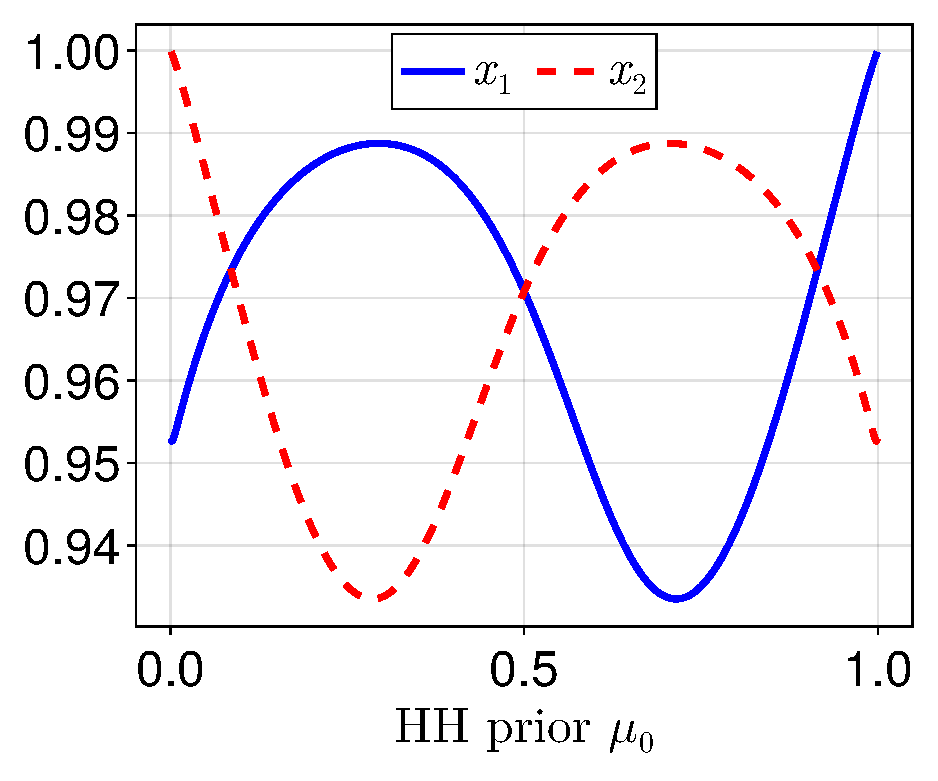
\includegraphics[width=0.49\textwidth]{figures/V11/γ=10.0-μ_0=0.5-α=1.0-θ=1.0-δ=0.5-ω_1=1.0-ω_2=-1.0/communication/fig_optimal_x_by_μ_0.pdf}
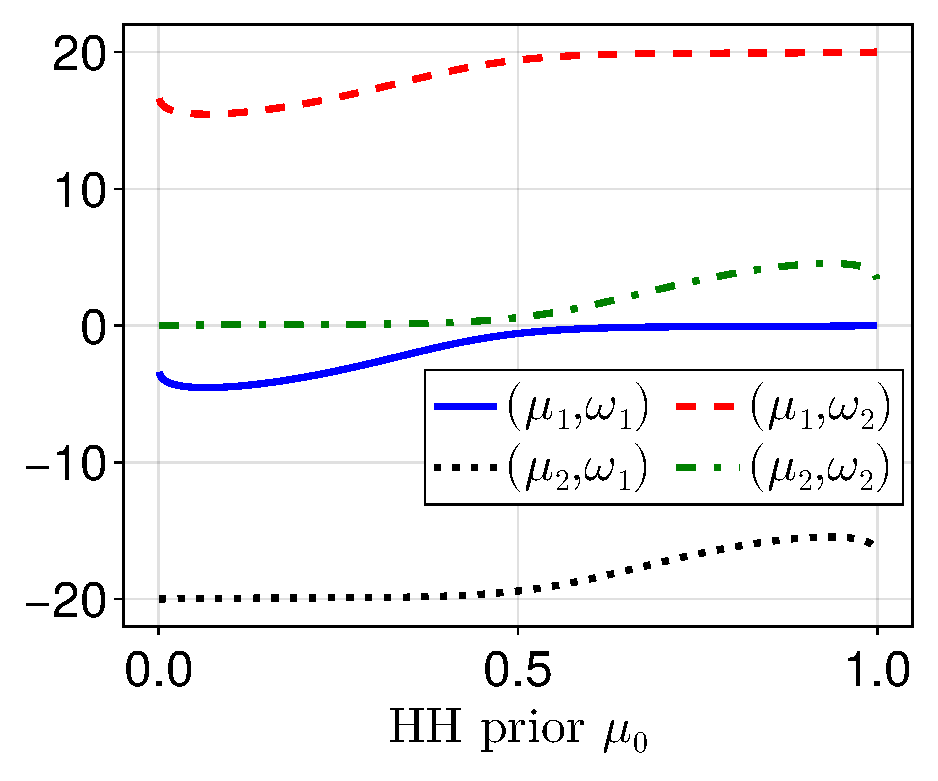
\includegraphics[width=0.49\textwidth]{figures/V11/γ=10.0-μ_0=0.5-α=1.0-θ=1.0-δ=0.5-ω_1=1.0-ω_2=-1.0/communication/fig_optimal_γ_by_μ_0.pdf}
\caption{Comparative statics for $\mu_0$ varying from 0 to 1, holding fixed all other parameters as in the benchmark.}
\label{Figure1}
\end{figure}

As Figure \ref{Figure1} shows, when HHs are either too optimistic or pessimistic, the effect on the information design is limited compared to the benchmark. CB's strategy is dominated by condition \eqref{threshold} dictating that, in the current scenario, inflation surprise is excessive and, thus, it is best for CB to remove uncertainty, although this will generate an unemployment gap. For instance, when HHs are mildly pessimistic (e.g., $\mu_0=0.7$), CB sets $x_2=1$ and $x_1$ smaller but close to 1. In other words, CB reveals whenever the negative shock (i.e., $\omega_1$) happens, while leaving some residual uncertainty on the positive shock (i.e., $\omega_2)$. Generalizing, CB focuses on eliminating the inflation surprise when the most plausible shock from the perspective of HHs realizes. This is likely due to the higher entropy cost associated with revealing the least plausible shock. Indeed, CB's intervention is not fully informative because of the presence of inattentive HHs. Increasing (decreasing) the share of inattentive HHs has the obvious effect of decreasing (increasing) the precision of CB's recommendations. This effect is asymmetric when HHs beliefs are not neutral, penalizing precision under the least plausible shock. See Figures \ref{FigureA1} and \ref{FigureA2} in the Appendix.

\begin{figure}[H]
\centering
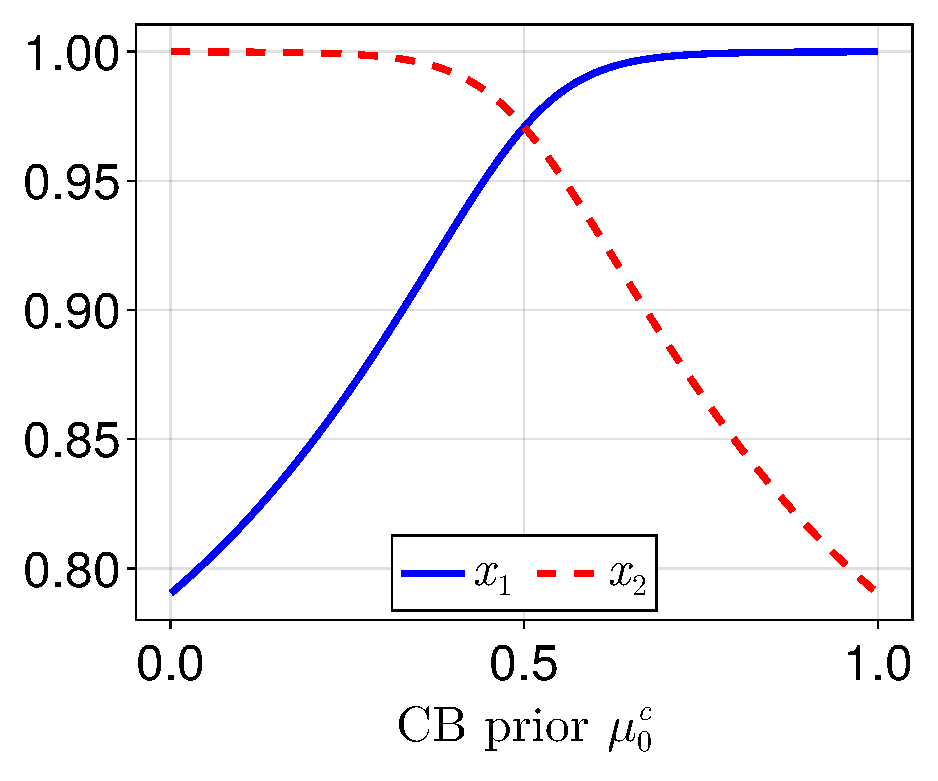
\includegraphics[width=0.49\textwidth]{figures/V11/γ=10.0-μ_0=0.5-α=1.0-θ=1.0-δ=0.5-ω_1=1.0-ω_2=-1.0/communication/fig_optimal_x_by_μ_0_c.pdf}
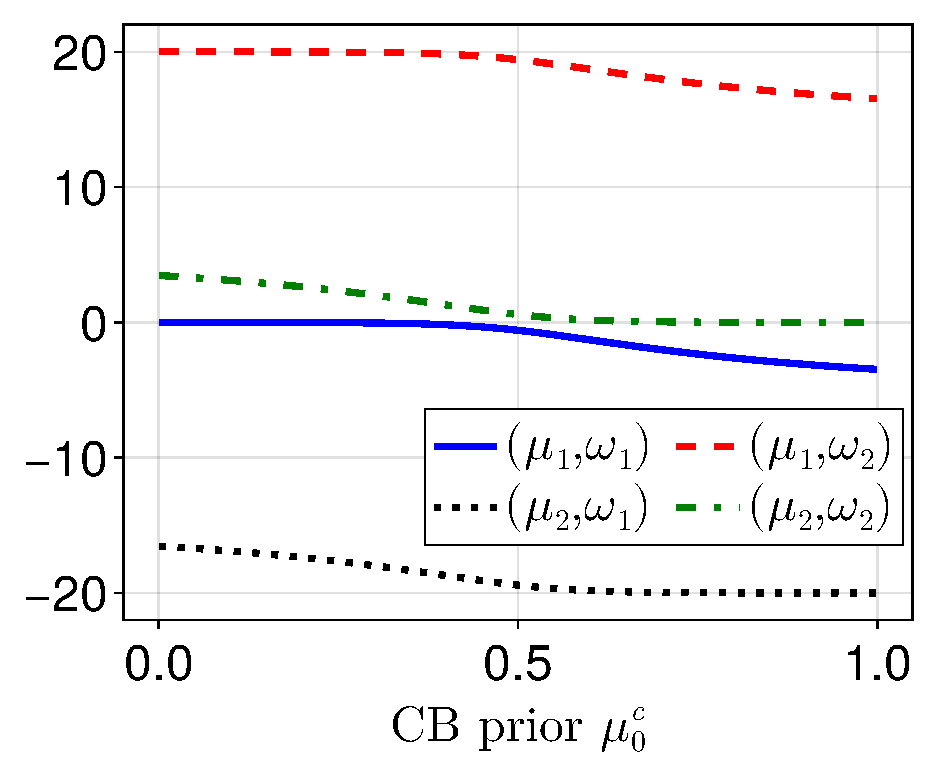
\includegraphics[width=0.49\textwidth]{figures/V11/γ=10.0-μ_0=0.5-α=1.0-θ=1.0-δ=0.5-ω_1=1.0-ω_2=-1.0/communication/fig_optimal_γ_by_μ_0_c.pdf}
\caption{Comparative statics for $\mu_0^c$ varying from 0 to 1, holding fixed all other parameters as in the benchmark.}
\label{Figure2}
\end{figure}

Figure \ref{Figure2} shows the effect of superior knowledge by the CB. In contrast to the effect of HHs optimism or pessimism, CB sacrifices precision of its recommendations concerning the shock that CB considers most plausible. The difference comes from the magnitude of inflation surprise, which is constant here, since $\mu_0=\frac{1}{2}$, whereas $\mu_0^c$ varies. For instance, when $\mu_0^c=0.7$, then $x_1=1$ whereas $x_2$ is smaller than 1. Equivalently, if CB believes a negative shock (i.e., $\omega_1$) to be more plausible, it will reveal whenever a positive shock (i.e., $\omega_2$) happens, while keeping some uncertainty on the negative shock. Indeed, given the presence of inattentive HHs, CB cannot completely eliminate inflation surprise. As before, this effect becomes more (less) prominent when the share of inattentive HHs increases (decreases). See Figures \ref{FigureA3} and \ref{FigureA4} in the Appendix.

\paragraph{Unemployment Shocks}
We are now interested in how asymmetric shocks come into play with belief heterogeneity, particularly the roles of shock magnitude and asymmetry. To this end, in contrast to the benchmark, where we consider $(\omega_1,\omega_2)=(1,-1)$, we further examine the effects of two extra cases: $(\omega_1,\omega_2)=(2,-2)$ and $(\omega_1,\omega_2)=(2,-1)$. The first case aims to study the role of shock magnitude, while the second checks the role of shock asymmetry. We then vary each HHs and CB priors at a time for the two cases and follow the same convention for reporting results. In other words, we redo the previous exercises with different shock combinations. The results are that neither shocks magnitude nor asymmetry play a significant role.
See Figures \ref{FigureA5}-\ref{FigureA8} in the Appendix. Remarkably, shocks play a role in the determining a discontinuity point in information design. See condition \eqref{threshold} and the results of the next section. Finally, we investigate how the effect of magnitude and asymmetry of shocks interact with the share of inattentive HHs. Our analysis confirms that shocks have only a limited impact on the precision of CB's information. See Figures \ref{FigureA9}-\ref{FigureA16} in the Appendix.


\subsection{Flatter Phillips Curve}
The flattened Phillips curve has become the new paradigm for interpreting the relationship between unemployment and inflation in recent years. It means the curve's inflation sensitivity $\gamma$ has approached one. This issue has become a major concern for policymakers on the effectiveness of monetary policy, especially while guiding the inflation expectation of market participants. To evaluate how such structural change affects the previous conclusions, we redo the same exercises as above with $\gamma=1$. Interestingly, when $\gamma=1$, this corresponds to the case when $4\omega > \gamma (\nu_1 + \nu_2)$, captured in Proposition \ref{Prop3}. Remarkably, our theoretical prediction for this scenario is that CB provides no information (or, equivalently, designs uninformative signals). This happens because the inflation surprise is relatively small and, in a condition of uncertainty by HHs, helps to reduce the impact of unemployment shocks. 

\paragraph{Heterogeneous Beliefs}
As before, we focus our analysis on the possibility that HHs and CB hold different prior beliefs. As Figure \ref{Figure3} shows, CB intervenes if HHs are either too optimistic or too pessimistic. In particular, in our benchmark where $\mu_0=\mu_0^c=\frac{1}{2}$, the inflation surprise exactly compensates for the shocks, thus implying a zero unemployment gap. This is the best scenario for the central bank and there is no reason to intervene. Consider, for instance, the possibility that HHs are instead too pessimistic (that is, $\mu_0\to 1$). There exists a threshold value of $\mu_0$ such that above it CB finds it optimal to send informative reports. In particular, above such threshold, $x_2=1$, implying that CB commits to revael to HHs whenever the negative shock (i.e., $\omega_1$) realizes. Why? Note that, as $\mu_0\to 1$, the inflation surprise becomes excessive in the case of a positive shock (i.e., $\omega_2$), whereas it is insufficient in the event of a negative shock. When this imbalance grows excessively, CB corrects it using signal $s_2$, which brings the inflation surprise closer to the optimal level. This comes at the cost of increasing the loss associated to $s_1$. Nevertheless, this is optimal for CB because $s_2$ occurs more often than $s_1$. Generalizing, CB responds to excessive optimism or pessimism by HHs inducing the optimal inflation surprise when the shock that HHs consider the least plausible realizes.

\begin{figure}[H]
\centering
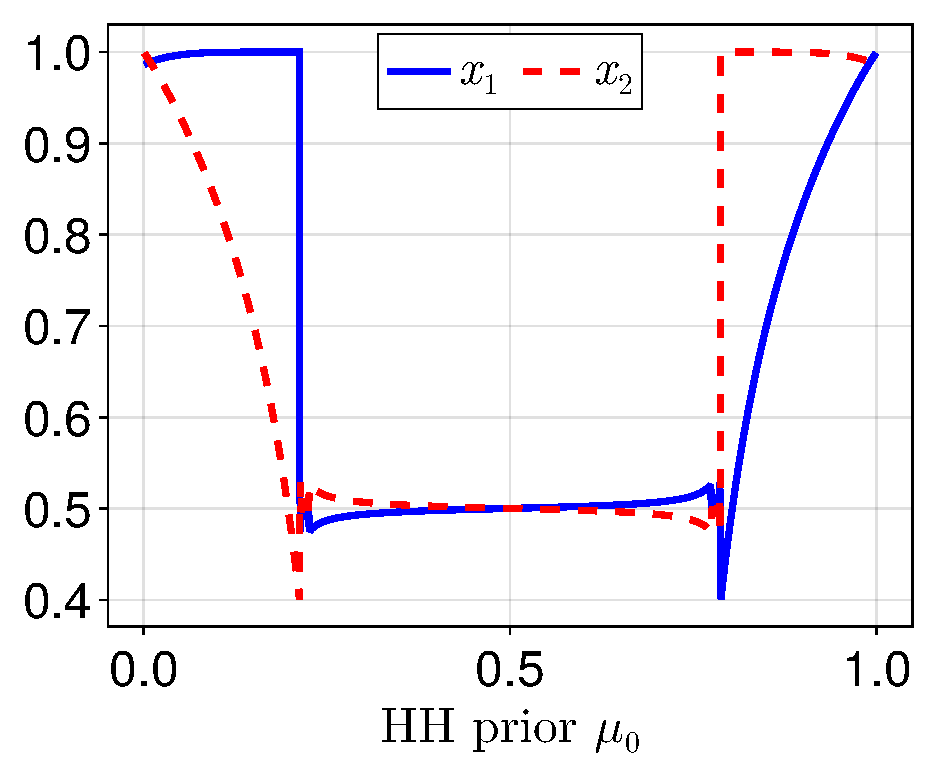
\includegraphics[width=0.49\textwidth]{figures/V11/γ=1.0-μ_0=0.5-α=1.0-θ=1.0-δ=0.5-ω_1=1.0-ω_2=-1.0/communication/fig_optimal_x_by_μ_0.pdf}
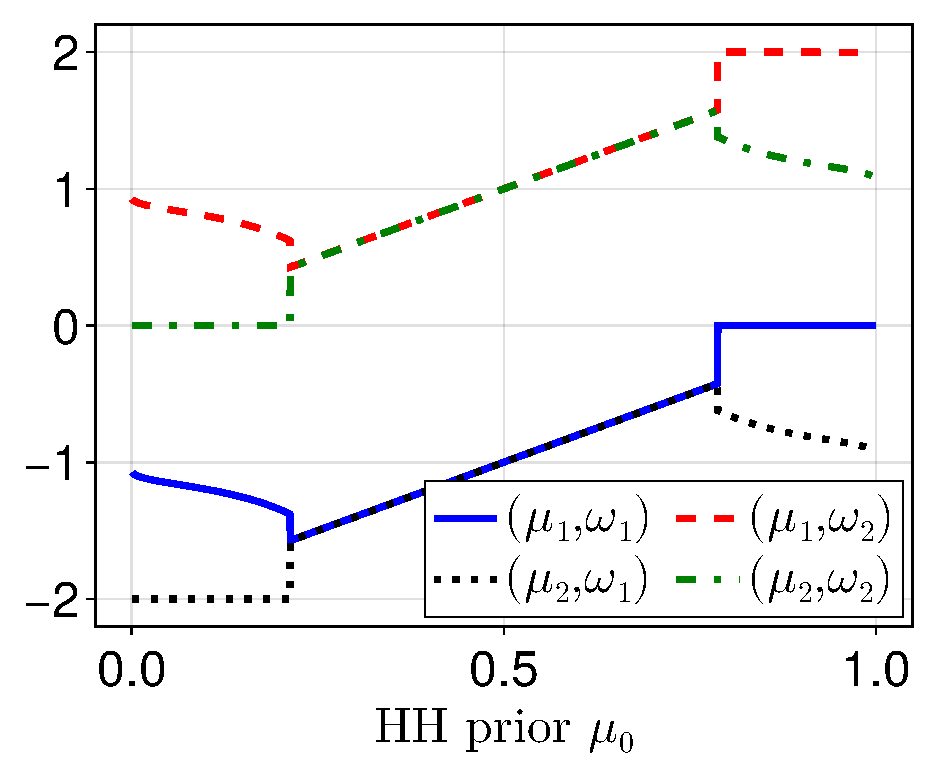
\includegraphics[width=0.49\textwidth]{figures/V11/γ=1.0-μ_0=0.5-α=1.0-θ=1.0-δ=0.5-ω_1=1.0-ω_2=-1.0/communication/fig_optimal_γ_by_μ_0.pdf}
\caption{Comparative statics for $\mu_0$ varying from 0 to 1, holding fixed all other parameters as in the benchmark.}
\label{Figure3}
\end{figure}

Instead, as Figure \ref{Figure4} shows, superior knowledge by CB has no impact on information design. As mentioned before, the reason is that inflation surprise is already at its optimal level given $\mu_0=\frac{1}{2}$. Thus, CB finds it optimal to provide no further information. CB's private information plays a role when HHs are optimistic or pessimistic. See Figure \ref{Figure4new}, where we assume that $\mu_0 = 0.1$, meaning that HHs are optimistic. CB intervenes when it does not share such optimism: when $\mu_0^c$ is above a threshold, CB sends informative reports. CB uses signal $s_1$ to return inflation surprise to its optimal value. This manipulation requires using signal $s_2$ to reveal when the economy is strong (i.e., $\omega_2$), which, however, comes with little surprise given HHs prior beliefs and makes this information design optimal. Therefore, our analysis shows that CB provides information when beliefs are sufficiently heterogeneous. 

 \begin{figure}[htp!]
    \centering
    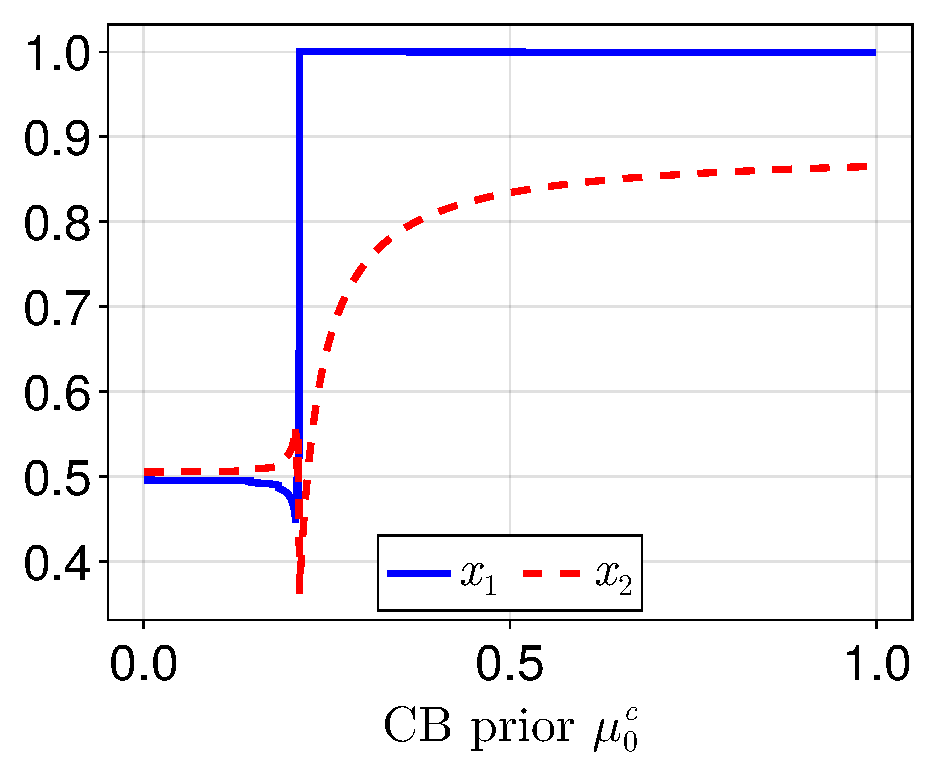
\includegraphics[width=0.49\textwidth]{figures/V11/γ=1.0-μ_0=0.1-α=1.0-θ=1.0-δ=0.5-ω_1=1.0-ω_2=-1.0/communication/fig_optimal_x_by_μ_0_c.pdf}
    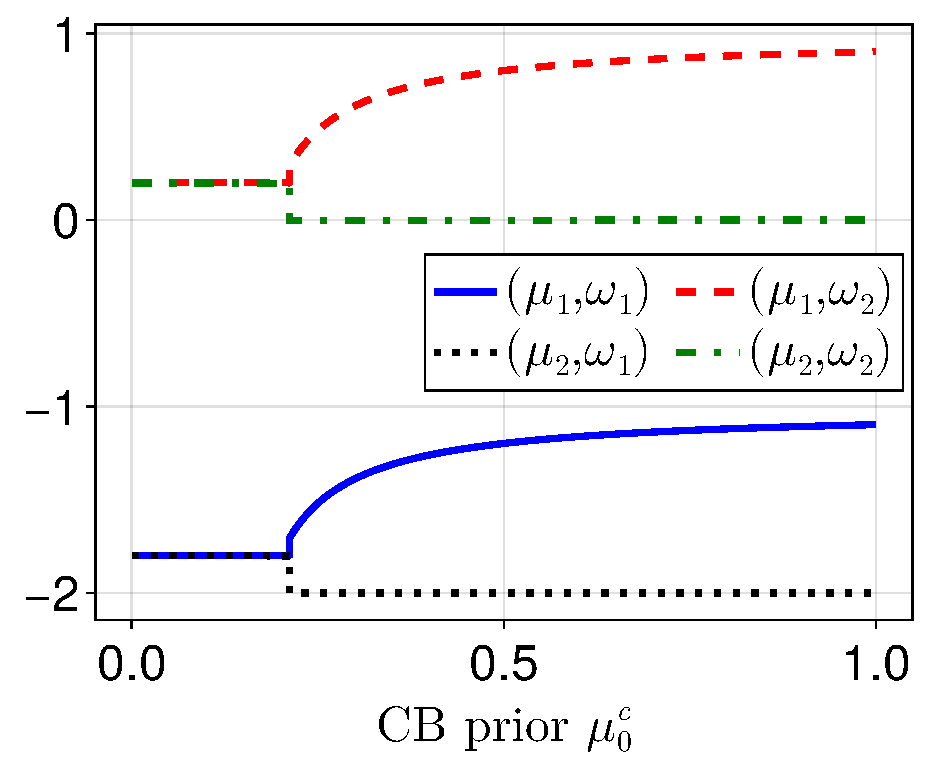
\includegraphics[width=0.49\textwidth]{figures/V11/γ=1.0-μ_0=0.1-α=1.0-θ=1.0-δ=0.5-ω_1=1.0-ω_2=-1.0/communication/fig_optimal_γ_by_μ_0_c.pdf}
    \caption{Comparative statics for $\mu_0^c$ varying from 0 to 1, assuming $\mu_0=0.1$ and holding fixed all other parameters as in the benchmark.}
    \label{Figure4new}
\end{figure}



\paragraph{Unemployment Shocks}
The magnitude and asymmetry of unemployment shocks change CB's response because they impact the optimality of inflation surprise in the benchmark. In particular, when $\mu_0=\frac{1}{2}$, the inflation surprise is insufficient, independently on the shock. Varying $\mu_0$ brings inflation surprise closer to the optimal level for one shock, but meanwhile away from the optimal level for the other shock. Information design cannot help CB in this scenario. See Figures \ref{FigureA17}-\ref{FigureA20} in the Appendix.


\paragraph{Share of Inattentive Households}
\label{sec:nu}
In this case, inattention does not play any significant role, neither alone nor in interaction with the magnitude and asymmetry of unemployment shocks. See Figures \ref{FigureA21}-\ref{FigureA32} in the Appendix.

\section{Optimal Flexibility in Asymmetric Scenarios} 
We now solve numerically central bank optimal choice of the monetary policy's flexibility $\nu$, prior to any communication. We use the same calibration as in the previous section. In Section \ref{sec:nu:compare}, we conduct comparative statics to better under the mechanisms of our model. In Section, \ref{sec:nu:interaction} we study the interaction between optimal flexibility and optimal communication by central bank.

\subsection{Comparative statics}
\label{sec:nu:compare}
We use as benchmark the parameters in Table \ref{tab:bchmrk_param}, which the exception of $\nu_1$ and $\nu_2$, which are now endogenous. As before, we consider different shapes of the Phillips curve (i.e., $\gamma=1$ and $\gamma=10$) and we vary all parameters one by one. Additionally, we also vary $\alpha$ - that is, the penalty associated with the inflation gap, which was irrelevant for information design - that in the benchmark is set equal to 1.

\begin{figure}[h!]
\centering
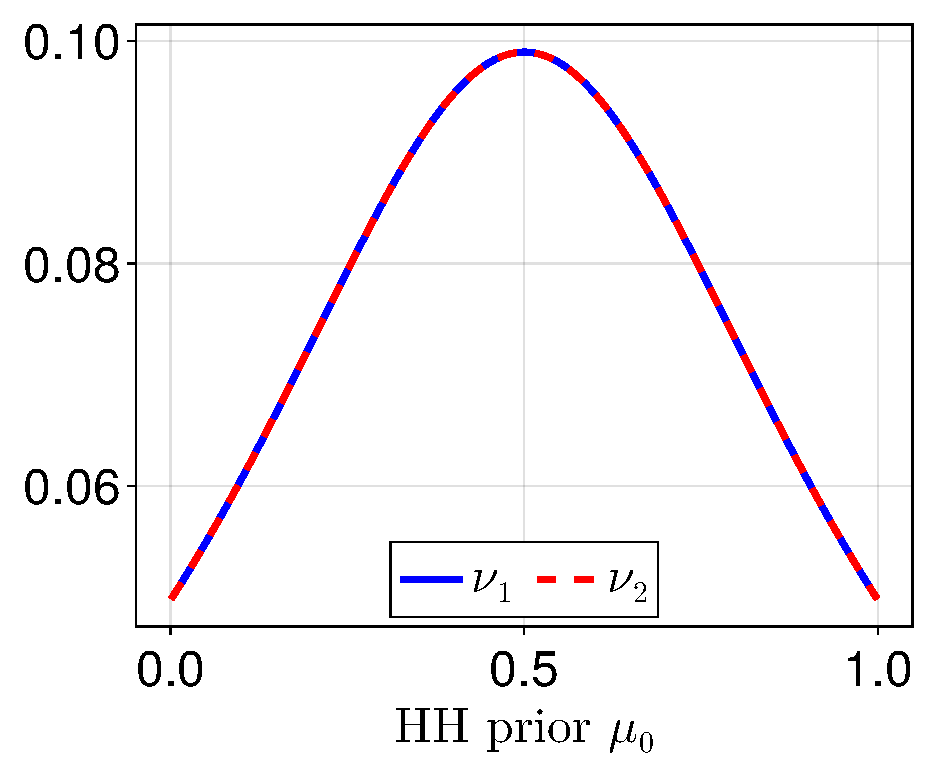
\includegraphics[width=0.49\textwidth]{figures/V11/γ=10.0-μ_0=0.5-α=1.0-θ=1.0-δ=0.5-ω_1=1.0-ω_2=-1.0/flexibility/fig_optimal_ν_by_μ_0.pdf}
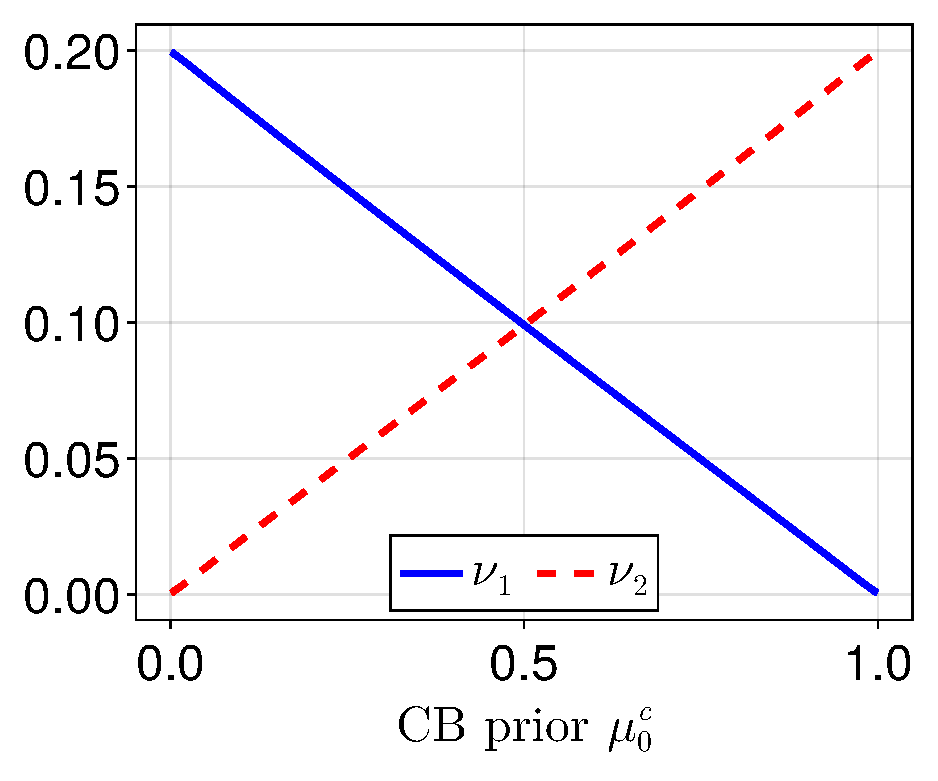
\includegraphics[width=0.49\textwidth]{figures/V11/γ=10.0-μ_0=0.5-α=1.0-θ=1.0-δ=0.5-ω_1=1.0-ω_2=-1.0/flexibility/fig_optimal_ν_by_μ_0_c.pdf}
\caption{Comparative statics for heterogeneous beliefs (either $\mu_0$ or $\mu_0^c$ varying from 0 to 1, holding fixed all other parameters as in the benchmark).}
\label{Figure5}
\end{figure}

We start considering $\gamma=10$ as in the benchmark. Figure \ref{Figure5} shows that when HHs becomes more certain about the state (in either direction), CB finds it optimal to allow for less flexibility. Flexibility is symmetric because $\nu_1$ and $\nu_2$ enter as a sum in the HHs' inflation expectation. Instead, when CB is more confident about the nature of the state, total flexibility is constant but CB allows more flexibility in the least likely state, so to reduce the expected inflation gap. Figure \ref{Figure6} shows that optimal flexibility increases in the total magnitude of the shocks, whereas the flexibility remains symmetric even when shocks are asymmetric. When $\gamma=1$, the relationship between optimal flexibility and the parameters is similar, as Figures \ref{FigureA33} and \ref{FigureA34} show. The only significant difference concerns the effect of $\mu_0^c$. When $\gamma=10$, the optimal flexibility is so small that the inflation gap does not play a significant role. Instead, when $\gamma=1$, the optimal flexibility is significantly constrained by its cost $\alpha$. If the CB becomes more certain about the state, it can allow more flexibility in the least likely state, approaching the optimal level in absence of cost associated with the inflation gap.

\begin{figure}[h!]
\centering
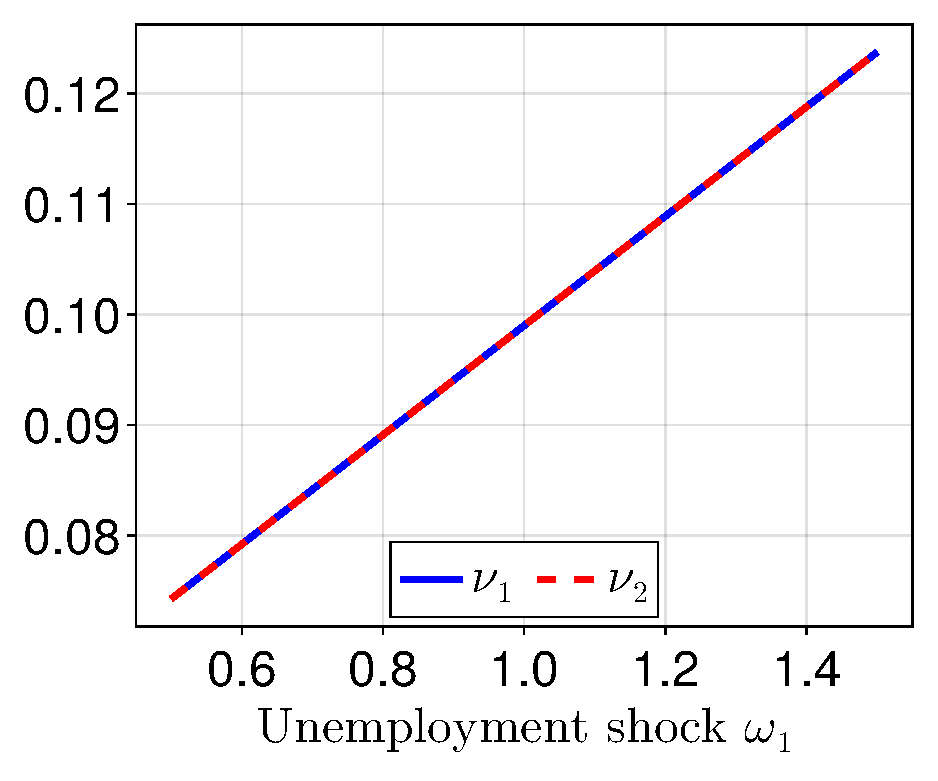
\includegraphics[width=0.49\textwidth]{figures/V11/γ=10.0-μ_0=0.5-α=1.0-θ=1.0-δ=0.5-ω_1=1.0-ω_2=-1.0/flexibility/fig_optimal_ν_by_ω_1.pdf}
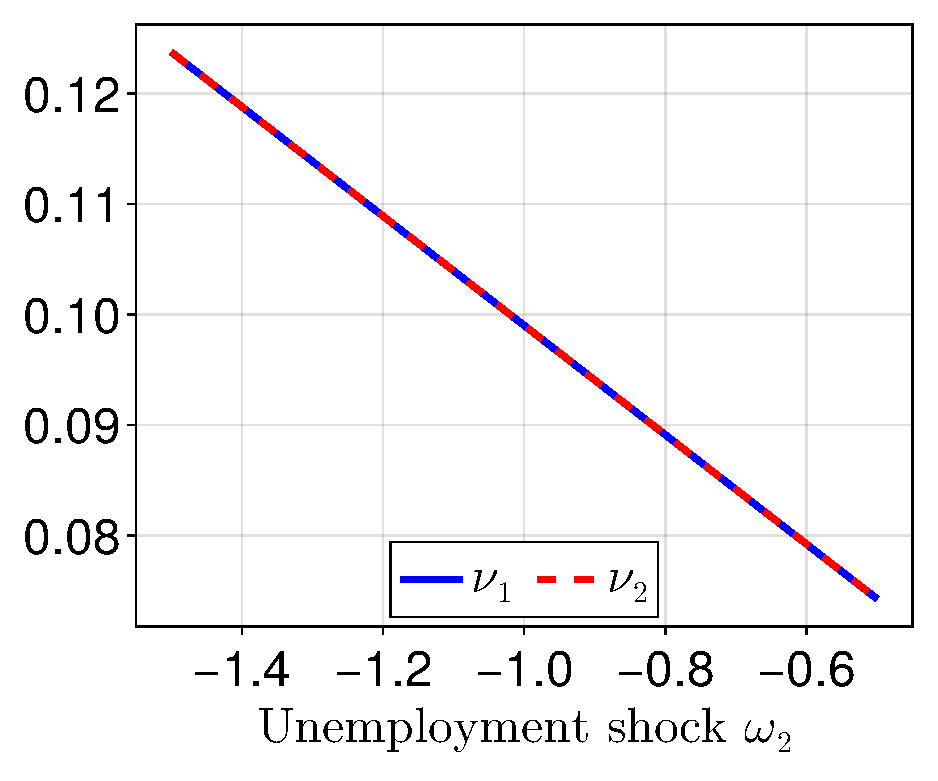
\includegraphics[width=0.49\textwidth]{figures/V11/γ=10.0-μ_0=0.5-α=1.0-θ=1.0-δ=0.5-ω_1=1.0-ω_2=-1.0/flexibility/fig_optimal_ν_by_ω_2.pdf}
\caption{Comparative statics for asymmetric shocks (either $\omega_1$ or $\omega_2$ vary, holding fixed all other parameters as in the benchmark).}
\label{Figure6}
\end{figure}

\subsection{Optimal communication given optimal flexibility}
\label{sec:nu:interaction}

In Section \ref{sec:bchmrk_res:comparative}, we have described how the central bank's information provision varies depending on the parameters for a given flexibility. In Section \ref{sec:nu:compare}, we show how the optimal flexibility depends on the same parameters. In this section, we combine the previous analyses. We find that information provision is always uninformative when the flexibility is optimal for a given set of parameters. Therefore, the result of the symmetric benchmark extends. When $\alpha=0$, this happens because optimal flexibility perfectly compensates for the shocks.
Instead, when $\alpha>0$, CB also considers the inflation gap, and thus, optimal flexibility is lower than what would be optimal for the unemployment gap. However, since flexibility reduces, this corresponds to the case where shocks are relatively large, and it is optimal to provide no information.
Therefore, information design is helpful only if the monetary policy's flexibility turns out to be excessive ex-post, which cannot happen in the equilibrium path.

\section{Extensions}

\subsection{Skewed HHs}
We consider an alternative distribution for the attention budget such that many HHs have a low attention budget, i.e., a right-skewed distribution of attention budget, and we analyze the impact of lower attention compared to the case where attention is uniformly distributed. In particular, we use the Kumaraswamy distribution, whose probability density function takes the following form:
\begin{align}
    f(x;a,b) & = a \cdot b \cdot x^{a-1} \cdot (1-x^a)^{b-1} \\
    F(x;a,b) & = 1 - (1-x^a)^b 
\end{align}
where $a$ and $b$ are non-negative shape parameters. This distribution collapses to a uniform distribution when $a=b=1$ and becomes right-skewed with $a=2$ and $b=5$. Our benchmark result (Proposition \ref{Prop3}) does not depend on the distribution of the attention budget. However, the latter has an effect when we consider asymmetric scenarios (Section \ref{sec:bchmrk_res}). In particular, we investigate how the shape parameters affect the effectiveness of central bank communication, e.g., $\partial \pi/ \partial a$.

\subsection{Irrational Inflation Expectations}
In this section, we relax Assumption \ref{Ass1}. In particular, we assume that beliefs are adaptive: 
$$\hat{\mu} = \mu_0 + \theta (\mu-\mu_0) = (1-\theta)\mu_0 + \theta \mu,$$
where $\theta\in[0,1]$.
\begin{lemma}
\label{adaptive}
    Adaptive belief and adaptive expectation are equivalent given the linear inflation expectation function $x^e$, where $\theta$ governs the extent to which information is used.
\end{lemma}

Under the symmetric benchmark---i.e., Assumptions \ref{Ass3} and \ref{Ass4} hold---the results do not differ qualitatively, as the next proposition shows.

\begin{proposition}
    \label{Prop4}
    Under Assumptions \ref{Ass1}-\ref{Ass4}, the solution to CB's information design problem depends on the inequality:
    \begin{equation}
    \label{threshold2}
        4\omega\geq\gamma(2-\theta)(\nu_1+\nu_2)
    \end{equation}
    If this holds then $x=\frac{1}{2}$. Otherwise, there is an interior solution. 
    The optimal flexibility provided by the CB is
    \begin{equation}
        \nu_1=\nu_2=\left(\frac{\gamma}{\gamma^2+\alpha}\right)\omega
    \end{equation}
    which implies that the optimal information design is uninformative.
\end{proposition}

\begin{figure}[H]
\centering
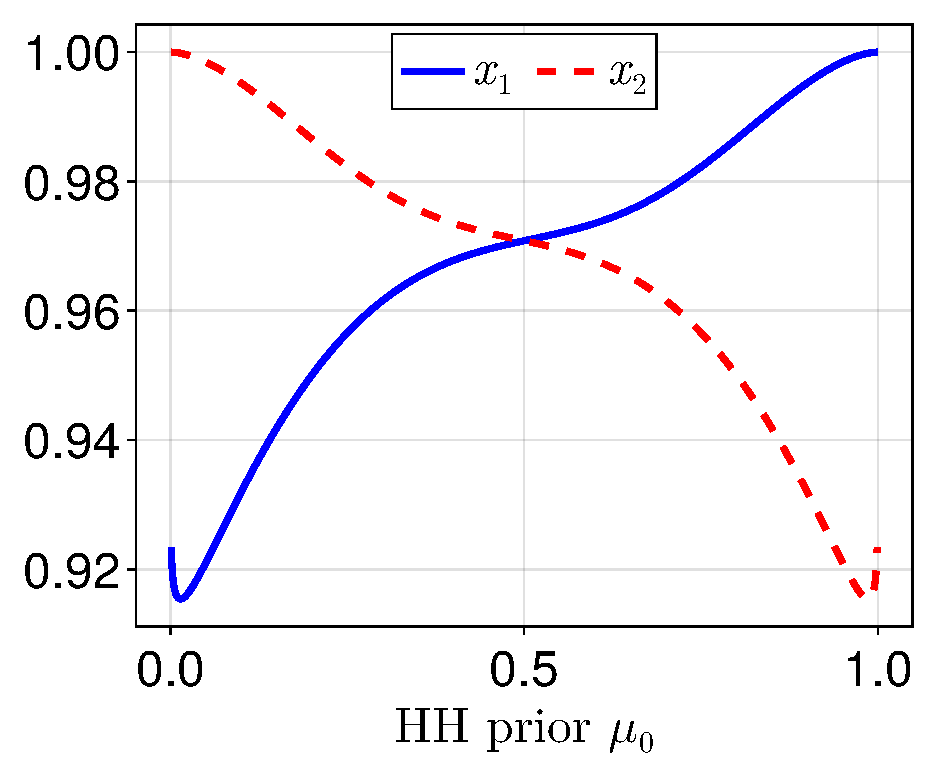
\includegraphics[width=0.49\textwidth]{figures/V11/γ=10.0-μ_0=0.5-α=1.0-θ=0.5-δ=0.5-ω_1=1.0-ω_2=-1.0/communication/fig_optimal_x_by_μ_0.pdf}
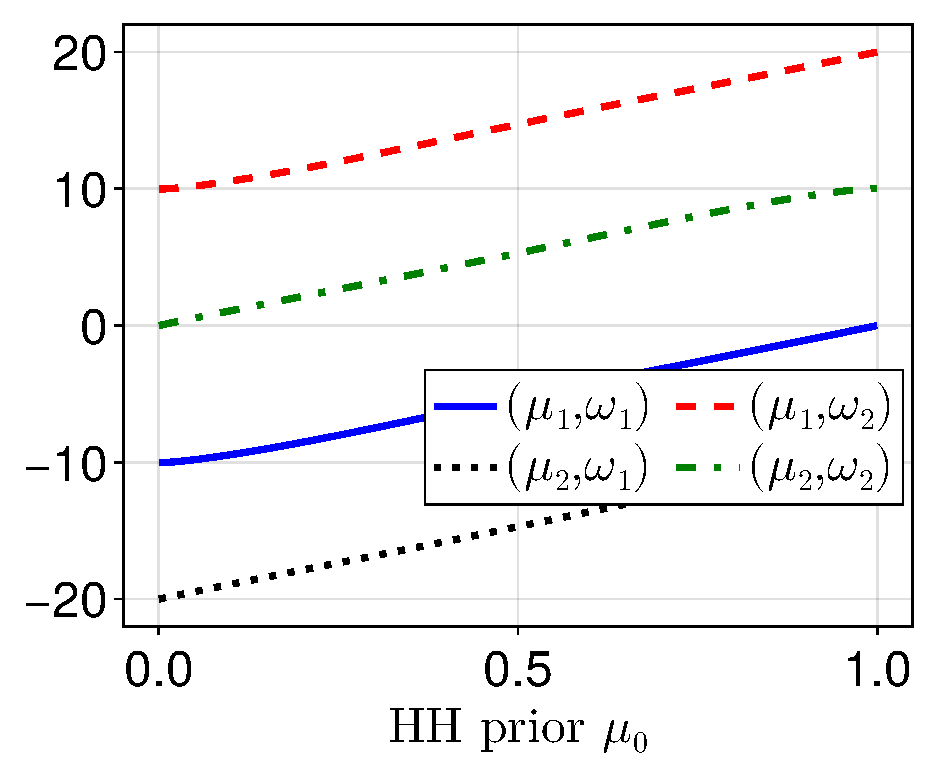
\includegraphics[width=0.49\textwidth]{figures/V11/γ=10.0-μ_0=0.5-α=1.0-θ=0.5-δ=0.5-ω_1=1.0-ω_2=-1.0/communication/fig_optimal_γ_by_μ_0.pdf}
\caption{Comparative statics for $\mu_0$ varying from 0 to 1 with $\theta = 0.5$, holding fixed all other parameters as in the benchmark.}
\label{Figure7}
\end{figure}


\subsection{Imperfect flexibility}

In this Section, we assume that CB cannot flexibly adjust to any possible realization of the negative shock. In particular, there are two possible realizations of the negative shock but CB can only vary its monetary policy based on the sign of the shock, as in the main model. However, CB can diversify its information policy based on the shock's magnitude.

Formally, the set of states becomes $\Omega \coloneqq \{\omega_1, \eta\omega_1,\omega_2\}$, with $\eta>0$.
The actual inflation, as a function of the state of the economy, becomes: 
\begin{equation}
    x(\omega,\nu)\coloneqq\left\{
    \begin{array}{cc}
      x^T+\nu_1&  \mbox{If } \omega=\omega_1 \mbox{ or } \omega=\eta\omega_1\\
      x^T-\nu_2   &  \mbox{If } \omega=\omega_2
    \end{array}
    \right.
\end{equation}
We also assume the following vectors of prior beliefs for HHs and CB, respectively: $\bar{\mu}_0\coloneqq\left(\frac{\mu_0}{2},\frac{\mu_0}{2},1-\mu_0\right)$ and $\bar{\mu}_0^c\coloneqq\left(\frac{\mu_0^c}{2},\frac{\mu_0^c}{2},1-\mu_0^c\right)$. The set of messages becomes $S=\{s_1,s_\eta,s_2\}$ and the vector of posterior beliefs for message $j$ is:
\begin{align}
    \mu_j = \left(\frac{\pi(s_j|\omega_1)\mu_0}{2\tau_j}, \frac{\pi(s_j|\eta\omega_1)\mu_0}{2\tau_j}, \frac{\pi(s_j|\omega_2)(1-\mu_0)}{2\tau_j}\right)
\end{align}
where
\begin{align}
    \tau_j = [\pi(s_j|\omega_1)+\pi(s_j|\eta\omega_1)]\frac{\mu_0}{2} + \pi(s_j|\omega_2)(1-\mu_0).
\end{align}
All the other elements of the main model do not change. Following \eqref{expected_uc}, CB solves the following minimization problem:
\begin{equation}
    \begin{split}
    \min_{\nu} \ & \ \delta F(c(\pi_\nu))\bar{\mu}_0^c\left\{\omega+\gamma\left[x^e(\bar{\mu}_0)-x(\omega,\nu)\right]\right\}^2+\\
    \ & \ +[1-\delta F(c(\pi_\nu))]\bar{\mu}_0^c\sum_{j=1}^{3}\pi_\nu(s_j|\omega)\left\{\omega+\gamma\left[x^e(\mu_j(\nu))-x(\omega,\nu)\right]\right\}^2+\\
    \ & \ +\alpha [\mu_0^c\nu_1^2+(1-\mu_0^c)\nu_2^2]
    \end{split}
\end{equation}
This problem is asymmetric by design. Therefore, we rely on numerical methods to solve it.

In addition to the uncertainty about the magnitude of the negative shock, CB may also face HHs who completely neglect such uncertainty. For instance, in the spirit of \cite{galperti2019persuasion}, we consider an alternative vector of prior belief for HHs: $\bar{\mu}_0\coloneqq\left(\mu_0,0,1-\mu_0\right)$. In particular, if the optimal $\pi$ reveals state $\eta \omega_1$, then HHs adopt the vector $\bar{\mu}_0\coloneqq\left(\frac{\mu_0}{2},\frac{\mu_0}{2},1-\mu_0\right)$ as prior beliefs.

Another possibility is to assume---in the spirit of \cite{evsyukova2024information}---that HHs are unaware of the existence of uncertainty about the negative shock. In particular, CB conceives all possible states in $\Omega$, whereas HHs conceive as state space $\Omega_{H}\coloneqq\{\bar{\omega}_1,\omega_2\}$, where $\bar{\omega}_1$ is a bundle of $\omega_1$ and $\eta\omega_1$, meaning that HHs cannot distinguish between these two. It follows that $\mu_0$ is the prior belief of $\bar{\omega}_1$ and two signals are sufficient, i.e., $S=\{s_1,s_2\}$. We consider the extreme scenario where HHs identify $\bar{\omega}_1$ with $\omega_1$, completely neglecting the possibility of the shock $\eta \omega_1$. As a result, CB can inflate any recommendation sending it in the event of a shock $\eta \omega_1$, since HHs would not account for the possibility of evidence being produced under such event.

\subsection{Uncertainty about Shock Magnitude}

In this Section, we assume that CB faces some uncertainty about the likelihood of shocks when choosing its monetary policy. In particular, in the first stage of the game, CB chooses its monetary policy---solving the problem in \eqref{minproblem2}---without knowing the exact likelihood of the shocks $\mu_0^c$. CB only knows that priors have distribution an atomless distribution $G(\cdot)$ with support $[0,1]$. Before the second stage, CB discovers its priors. Therefore, CB can use information design to correct a wrongly specified monetary policy. Since CB knows its priors, the information design stage is the same as in the main analysis. We thus focus on the response of the monetary policy to uncertainty, and the implications for CB's communication strategy. Our numerical analysis shows that



\section{Conclusion}

This paper studies the optimal information design of a central bank, which also controls inflation through its monetary policy.
We find that communication is a tool the central bank uses only when its monetary policy is sub-optimal given the economic fundamentals. In particular, the central bank provides information if the flexibility is excessive; that is, the magnitude of the unemployment shock is small, and thus, the inflation surprise is excessive, making it optimal to remove uncertainty about the state of the economy. Alternatively, the central bank provides information if the shock is relatively large, but households are either too optimistic or too pessimistic, making the inflation surprise excessive when the state that households consider unlikely realizes. In all other cases, the central bank finds it optimal to remain silent. Our results can rationalize the ``whatever it takes'' statement by Mario Draghi. The ECB was facing a significant unemployment shock. Thus, using the inflation surprise generated by allowed flexibility to smooth the shock is optimal. By contrast, revealing the state of the economy and thus eliminating inflation surprise could not help reduce the shock's harmful effects.

\newpage
\bibliographystyle{ecta}
\bibliography{references}

\appendix

\section{Mathematical details}
\label{math}
We denote with $x_1=\pi(s_1|\omega_1)$ and $x_2=\pi(s_2|\omega_2)$. It follows that:
\begin{align}
    \mu_1 & = \frac{x_1\mu_0}{x_1\mu_0 + (1-x_2)(1-\mu_0)} \\
    \mu_2 & = \frac{(1-x_1)\mu_0}{(1-x_1)\mu_0 + x_2(1-\mu_0)}\\
    \frac{\partial \mu_1}{\partial x_1} & =\frac{\mu_0(1-\mu_0)(1-x_2)}{[x_1\mu_0+(1-x_2)(1-\mu_0)]^2}\\
    \frac{\partial \mu_2}{\partial x_1} & =\frac{-\mu_0(1-\mu_0)x_2}{[(1-x_1)\mu_0+x_2(1-\mu_0)]^2}\\
    \frac{\partial \mu_1}{\partial x_2} & =\frac{\mu_0(1-\mu_0)x_1}{[x_1\mu_0+(1-x_2)(1-\mu_0)]^2}\\
    \frac{\partial \mu_2}{\partial x_2} & =\frac{-\mu_0(1-\mu_0)(1-x_1)}{[(1-x_1)\mu_0+x_2(1-\mu_0)]^2} \\
    \tau_1 & =x_1\mu_0 + (1-x_2)(1-\mu_0) \\
    \tau_2 & =(1-x_1)\mu_0 + x_2(1-\mu_0) \\
    \frac{\partial \tau_{j}}{\partial x_1} & = \left\{\begin{array}{ll}
        \mu_0 & \mbox{if } j = 1\\
        -\mu_0 & \mbox{otherwise}
        \end{array}\right. \\
        \frac{\partial \tau_{j}}{\partial x_2} & = \left\{\begin{array}{ll}
        1-\mu_0 & \mbox{if } j = 2\\
        -(1-\mu_0) & \mbox{otherwise}
        \end{array}\right. \\
    \frac{\partial H(\mu_{j})}{\partial x_k} & = -\frac{\partial \mu_j}{\partial x_k}\ln\left(\frac{\mu_j}{1-\mu_j}\right) \\
    c_k^\prime(\pi) & = -\chi \sum_{j=1,2} \left[\frac{\partial \tau_{j}}{\partial x_k}H(\mu_j) + \tau_{j}\frac{\partial H(\mu_j)}{\partial x_k}\right]
\end{align}

\paragraph{Proof of Proposition \ref{Prop3}}
The F.O.C. are:
\begin{small}
\begin{equation}
    \begin{split}
        \delta f(c(\pi))c_1^\prime(\pi)\Bigg\{\mu_0^c\left[\omega_1-\gamma(\nu_1+\nu_2)(1-\mu_0)\right]^2+(1-\mu_0^c)\left[\omega_2+\gamma(\nu_1+\nu_2)\mu_0\right]^2\Bigg\}+ &\\
        -\delta f(c(\pi))c_1^\prime(\pi)\Bigg\{\mu_0^c\bigg[x_1(\omega_1-\gamma (\nu_1+\nu_2) (1-\mu_1))^2+(1-x_1)(\omega_1-\gamma (\nu_1+\nu_2) (1-\mu_2))^2\bigg]+ & \\
        +(1-\mu_0^c)\bigg[x_2(\omega_2+\gamma (\nu_1+\nu_2) \mu_2)^2+(1-x_2)(\omega_2+\gamma (\nu_1+\nu_2) \mu_1)^2 \bigg]\Bigg\}+ & \\
        +[1-\delta F(c(\pi))]\Bigg\{\mu_0^c\Bigg[(\omega_1-\gamma(\nu_1+\nu_2)(1-\mu_1))^2+2x_1(\omega_1-\gamma(\nu_1+\nu_2)(1-\mu_1))\gamma(\nu_1+\nu_2)\frac{\partial \mu_1}{\partial x_1}+ & \\
        -(\omega_1-\gamma(\nu_1+\nu_2)(1-\mu_2))^2+2(1-x_1)(\omega_1-\gamma(\nu_1+\nu_2)(1-\mu_2))\gamma(\nu_1+\nu_2)\frac{\partial \mu_2}{\partial x_1}\Bigg]+ &\\
        +2\gamma(\nu_1+\nu_2)(1-\mu_0^c)\left[x_2(\omega_2+\gamma(\nu_1+\nu_2)\mu_2)\frac{\partial \mu_2}{\partial x_1}+(1-x_2)(\omega_2+\gamma(\nu_1+\nu_2)\mu_1)\frac{\partial \mu_1}{\partial x_1}\right]\Bigg\} & =0
    \end{split} 
\end{equation}
\begin{equation}
    \begin{split}
    \delta f(c(\pi))c_2^\prime(\pi)\Bigg\{\mu_0^c\left[\omega_1-\gamma(\nu_1+\nu_2)(1-\mu_0)\right]^2+(1-\mu_0^c)\left[\omega_2+\gamma(\nu_1+\nu_2)\mu_0\right]^2\Bigg\}+ &\\
    -\delta f(c(\pi))c_2^\prime(\pi)\Bigg\{\mu_0^c\bigg[x_1(\omega_1-\gamma (\nu_1+\nu_2) (1-\mu_1))^2+(1-x_1)(\omega_1-\gamma (\nu_1+\nu_2) (1-\mu_2))^2\bigg]+ & \\
    +(1-\mu_0^c)\bigg[x_2(\omega_2+\gamma (\nu_1+\nu_2) \mu_2)^2+(1-x_2)(\omega_2+\gamma (\nu_1+\nu_2) \mu_1)^2 \bigg]\Bigg\}+ & \\
    +[1-\delta F(c(\pi))]\Bigg\{
    (1-\mu_0^c)\Bigg[(\omega_2+\gamma(\nu_1+\nu_2)\mu_2)^2+2x_2(\omega_2+\gamma(\nu_1+\nu_2)\mu_2)\gamma(\nu_1+\nu_2)\frac{\partial \mu_2}{\partial x_2}+ & \\
    -(\omega_2+\gamma(\nu_1+\nu_2)\mu_1)^2+2(1-x_2)(\omega_2+\gamma(\nu_1+\nu_2)\mu_1)\gamma(\nu_1+\nu_2)\frac{\partial \mu_1}{\partial x_2}\Bigg]+ & \\
    +2\gamma(\nu_1+\nu_2)\mu_0^c\left[x_1(\omega_1-\gamma(\nu_1+\nu_2)(1-\mu_1))\frac{\partial \mu_1}{\partial x_2}+(1-x_1)(\omega_1-\gamma(\nu_1+\nu_2)(1-\mu_2))\frac{\partial \mu_2}{\partial x_2}\right]\Bigg\} & =0
    \end{split}
\end{equation}
\end{small}
Applying assumptions \ref{Ass3}-\ref{Ass4}, the F.O.C.s becomes symmetric. Thus, we consider symmetric solutions where $x_1=x_2=x$.
It follows that the solution to the CB's information design problem solves the following condition:
    \begin{equation}
    \label{focdeltanonzero}
        \gamma(\nu_1+\nu_2)[4\omega-\gamma(\nu_1+\nu_2)]\left\{[1-\delta F(c(\pi))](2x-1)+2\delta f(c(\pi))c^\prime(\pi)\left[x(1-x)-\frac{1}{4}\right]\right\}=0
    \end{equation}
    where
    \begin{eqnarray}
        c(\pi)=\chi \left[\ln(2)+x\ln(x)+(1-x)\ln(1-x)\right] \\
        c^\prime(\pi)=\frac{\chi}{2}\left[\ln\left(x\right)-\ln(1-x)\right]
    \end{eqnarray}
    Since
    \begin{eqnarray}
        2\delta f(c(\pi))c^\prime(\pi)\left[x(1-x)-\frac{1}{4}\right]\leq 0 \quad \forall x\in\left[\frac{1}{2},1\right] \\
        \lim_{x\to 1}2\delta f(c(\pi))c^\prime(\pi)\left[x(1-x)-\frac{1}{4}\right]=-\infty \\
        \lim_{x\to\frac{1}{2}}[1-\delta F(c(\pi))](2x-1)+2\delta f(c(\pi))c^\prime(\pi)\left[x(1-x)-\frac{1}{4}\right]=0
    \end{eqnarray}
    If there exists an interior solution to \eqref{focdeltanonzero}, then it must be a maximum point, provided that $4\omega-\gamma(\nu_1+\nu_2)\geq0$. Therefore, CB's problem has a corner solution: either $x=\frac{1}{2}$ or $x=1$. CB's utility when $x=\frac{1}{2}$ is
    \begin{equation}
        u_{x=\frac{1}{2}}=-\left[\omega-\frac{\gamma}{2}(\nu_1+\nu_2)\right]^2
    \end{equation}
    whereas CB's utility when $x=1$ is
    \begin{equation}
        u_{x=1}=-\delta\left[\omega-\frac{\gamma}{2}(\nu_1+\nu_2)\right]^2-(1-\delta)\omega^2
    \end{equation}
Comparing these two, we observe that CB's utility is higher with $x=\frac{1}{2}$ if and only if
\begin{equation}
\label{constraintomega}
    \left[\omega-\frac{\gamma}{2}(\nu_1+\nu_2)\right]^2\leq \omega^2 \iff \omega\geq \frac{\gamma}{4}(\nu_1+\nu_2)
\end{equation}
Following \eqref{minproblem2}, the optimal flexibility given $x=\frac{1}{2}$ solves:
\begin{equation}
    \begin{split}
    \min_{\{\nu_1,\nu_2\}} \ & \ \left(\omega-\frac{\gamma}{2}(\nu_1+\nu_2)\right)^2
    +\frac{\alpha}{2}(\nu_1^2+\nu_2^2)
    \end{split}
\end{equation}
The F.O.C.s are:
\begin{eqnarray}
2\left(\omega-\frac{\gamma}{2}(\nu_1+\nu_2)\right)\left(-\frac{\gamma}{2}\right)+\alpha \nu_1=0\\
2\left(\omega-\frac{\gamma}{2}(\nu_1+\nu_2)\right)\left(-\frac{\gamma}{2}\right)+\alpha \nu_2=0
\end{eqnarray}
Since the F.O.C.s are symmetric, the solution is symmetric:
\begin{equation}
\label{optflex}
    \nu_1=\nu_2=\nu=\left(\frac{\gamma}{\gamma^2+\alpha}\right)\omega
\end{equation}
The problem is correctly specified since
\begin{equation}
    \omega\geq\frac{\gamma}{4} (\nu_1+\nu_2)=\left(\frac{\gamma^2}{2(\gamma^2+\alpha)}\right)\omega 
\end{equation}
which satisfies \eqref{constraintomega}. When \eqref{constraintomega} does not hold, there can be an interior solution to \eqref{focdeltanonzero}. CB's utility with a generic symmetric solution $x\in\left[\frac{1}{2},1\right]$ is:
\begin{equation}
    \begin{split}
        u_{x}= & \, -\delta F(c(\pi))\left[\omega-\frac{\gamma}{2}(\nu_1+\nu_2)\right]^2+\\
        & -[1-\delta F(c(\pi))]\left[x(\omega-\gamma(\nu_1+\nu_2)(1-x))^2+(1-x)(\omega-\gamma(\nu_1+\nu_2)x)^2\right]
    \end{split}
\end{equation}
We verify that $u_x\geq u_{x=\frac{1}{2}}$ if and only if \eqref{constraintomega} does not hold. Assume, for simplicity, $F(\cdot)=U[0,1]$. Following \eqref{focdeltanonzero}, the optimal precision of information $x$ solves:
\begin{equation}
    [1-\delta\chi\ln(2)](2x-1)+\delta\chi \left[\ln(x)\left(2x-3x^2-\frac{1}{4}\right)+\ln(1-x)\left(3x^2-4x+\frac{5}{4}\right)\right]=0
\end{equation}
There exists a threshold value $\hat{\delta}$ such that $x=1$ for any $\delta\leq \hat{\delta}$, whereas $x\in\left(\frac{1}{2},1\right)$ for any $\delta>\hat{\delta}$. Remarkably, the solution $x$ to \eqref{focdeltanonzero} does not depend on $\nu_1$ and $\nu_2$. The CB's problem in the first stage is:
\begin{equation}
    \begin{split}
    \min_{\{\nu_1,\nu_2\}} \ & \ -u_x
    +\frac{\alpha}{2}(\nu_1^2+\nu_2^2)
    \end{split}
\end{equation}
The corresponding F.O.C.s are:
\begin{eqnarray}
2\delta c(\pi)\left(\omega-\frac{\gamma}{2}(\nu_1+\nu_2)\right)\left(-\frac{\gamma}{2}\right)+2[1-\delta c(\pi)]\left[x(1-x)(2\omega-\gamma(\nu_1+\nu_2))\right](-\gamma)+\alpha \nu_1=0\\
2\delta c(\pi)\left(\omega-\frac{\gamma}{2}(\nu_1+\nu_2)\right)\left(-\frac{\gamma}{2}\right)+2[1-\delta c(\pi)]\left[x(1-x)(2\omega-\gamma(\nu_1+\nu_2))\right](-\gamma)+\alpha \nu_2=0
\end{eqnarray}
The F.O.C.s are symmetric. Thus, $\nu_1=\nu_2=\nu$, which implies:
\begin{equation}
\label{focsymmetricv}
    -\gamma\delta c(\pi)\left(\omega-\gamma \nu\right)-4\gamma[1-\delta c(\pi)]\left[x(1-x)(\omega-\gamma \nu)\right]+\alpha \nu=0
\end{equation}
Therefore, the optimal flexibility $\hat{\nu}$ solving \eqref{focsymmetricv} is:
\begin{equation}
    \hat{\nu}=\left(\frac{\gamma \left\{4x(1-x)+\delta c(\pi)[1-4x(1-x)]\right\}}{\gamma^2\left\{4x(1-x)+\delta c(\pi)[1-4x(1-x)] \right\}+\alpha }\right)\omega
\end{equation}
When $\nu_1=\nu_2=\hat{\nu}$, the condition \eqref{constraintomega} holds, thus contradicting the initial assumption. We conclude that a partially or fully informative $\pi$ cannot be part of the equilibrium path. For CB, it is optimal to give flexibility $\nu$ as in \eqref{optflex} and, then, provide no information.

\paragraph{Proof of Lemma \ref{adaptive}}

\begin{proof}
    \begin{align*}
        x^e(\hat{\mu}) &= x^T+\nu_1\hat{\mu}-\nu_2(1-\hat{\mu}) \\
        &= x^T + \nu_1\left((1-\theta)\mu_0 + \theta\mu\right) - \nu_2\left(1-(1-\theta)\mu_0 - \theta\mu\right) \\
        &= x^T + \nu_1(1-\theta)\mu_0 + \nu_1\theta\mu - \nu_2 + \nu_2(1-\theta)\mu_0 + \nu_2\theta\mu \\
        & = (1-\theta)x^T + \theta x^T + \nu_1(1-\theta)\mu_0 + \nu_1\theta\mu - (1-\theta)\nu_2 - \theta\nu_2 + \nu_2(1-\theta)\mu_0 + \nu_2\theta\mu \\
        &= (1-\theta)\left[x^T + \nu_1\mu_0-\nu_2(1-\mu_0)\right] + \theta\left[x^T + \nu_1\mu-\nu_2(1-\mu)\right] \\
        &= (1-\theta)x^e(\mu_0) + \theta x^e(\mu) \\
        &= \hat{x}^e
    \end{align*}
\end{proof}

\paragraph{Proof of Proposition \ref{Prop4}}

Under adaptive belief, the second-stage problem in \eqref{minproblem} becomes:
\begin{footnotesize}
\begin{equation}
\begin{split}
    \min_{\pi} \ & \ \delta F(c(\pi))\Bigg\{\mu_0^c\left[\omega_1-\gamma(\nu_1+\nu_2)(1-\mu_0)\right]^2+(1-\mu_0^c)\left[\omega_2+\gamma(\nu_1+\nu_2)\mu_0\right]^2\Bigg\}+\\
    \ & \ +[1-\delta F(c(\pi))]\Bigg\{\mu_0^c\bigg[\pi(s_1|\omega_1)(\omega_1-\gamma \left(\nu_1(1-(1-\theta)\mu_0-\theta\mu_1)+\nu_2((1-\theta)(1-\mu_0)+\theta(1-\mu_1))\right))^2+\\
    \ & \ +\pi(s_2|\omega_1)(\omega_1-\gamma \left(\nu_1(1-(1-\theta)\mu_0-\theta\mu_2)+\nu_2((1-\theta)(1-\mu_0)+\theta(1-\mu_2))\right))^2\bigg]+ \\
    \ & \ +(1-\mu_0^c)\bigg[\pi(s_2|\omega_2)(\omega_2+\gamma \left(\nu_1((1-\theta)\mu_0+\theta\mu_2)+\nu_2(1-(1-\theta)(1-\mu_0)-\theta(1-\mu_2))\right))^2+\\
    \ & \ +\pi(s_1|\omega_2)(\omega_2+\gamma \left(\nu_1((1-\theta)\mu_0+\theta\mu_1)+\nu_2(1-(1-\theta)(1-\mu_0)-\theta(1-\mu_1))\right))^2 \bigg]\Bigg\}
    \end{split}
\end{equation}
\end{footnotesize}

The F.O.C. are:
\begin{footnotesize}
\begin{equation}
    \begin{split}
        \delta f(c(\pi))c_1^\prime(\pi)\Bigg\{\mu_0^c\left[\omega_1-\gamma(\nu_1+\nu_2)(1-\mu_0)\right]^2+(1-\mu_0^c)\left[\omega_2+\gamma(\nu_1+\nu_2)\mu_0\right]^2\Bigg\}+ &\\
        -\delta f(c(\pi))c_1^\prime(\pi)\Bigg\{\mu_0^c\bigg[x_1(\omega_1-\gamma \left(\nu_1(1-(1-\theta)\mu_0-\theta\mu_1)+\nu_2((1-\theta)(1-\mu_0)+\theta(1-\mu_1))\right))^2+ &\\
        +(1-x_1)(\omega_1-\gamma \left(\nu_1(1-(1-\theta)\mu_0-\theta\mu_2)+\nu_2((1-\theta)(1-\mu_0)+\theta(1-\mu_2))\right))^2\bigg]+ &\\
        +(1-\mu_0^c)\bigg[x_2(\omega_2+\gamma \left(\nu_1((1-\theta)\mu_0+\theta\mu_2)+\nu_2(1-(1-\theta)(1-\mu_0)-\theta(1-\mu_2))\right))^2+ &\\
        +(1-x_2)(\omega_2+\gamma \left(\nu_1((1-\theta)\mu_0+\theta\mu_1)+\nu_2(1-(1-\theta)(1-\mu_0)-\theta(1-\mu_1))\right))^2 \bigg]\Bigg\}+ & \\
        +[1-\delta F(c(\pi))]\Bigg\{\mu_0^c\Bigg[(\omega_1-\gamma \left(\nu_1(1-(1-\theta)\mu_0-\theta\mu_1)+\nu_2((1-\theta)(1-\mu_0)+\theta(1-\mu_1))\right))^2+ & \\
        +2x_1(\omega_1-\gamma \left(\nu_1(1-(1-\theta)\mu_0-\theta\mu_1)+\nu_2((1-\theta)(1-\mu_0)+\theta(1-\mu_1))\right))\gamma\theta(\nu_1+\nu_2)\frac{\partial \mu_1}{\partial x_1}+ & \\
        -(\omega_1-\gamma \left(\nu_1(1-(1-\theta)\mu_0-\theta\mu_2)+\nu_2((1-\theta)(1-\mu_0)+\theta(1-\mu_2))\right))^2+ & \\
        +2(1-x_1)(\omega_1-\gamma \left(\nu_1(1-(1-\theta)\mu_0-\theta\mu_2)+\nu_2((1-\theta)(1-\mu_0)+\theta(1-\mu_2))\right))\gamma\theta(\nu_1+\nu_2)\frac{\partial \mu_2}{\partial x_1}\Bigg]+ &\\
        +2\gamma\theta(\nu_1+\nu_2)(1-\mu_0^c)\Bigg[x_2(\omega_2+\gamma \left(\nu_1((1-\theta)\mu_0+\theta\mu_2)+\nu_2(1-(1-\theta)(1-\mu_0)-\theta(1-\mu_2))\right))\frac{\partial \mu_2}{\partial x_1}+ & \\
        +(1-x_2)(\omega_2+\gamma \left(\nu_1((1-\theta)\mu_0+\theta\mu_1)+\nu_2(1-(1-\theta)(1-\mu_0)-\theta(1-\mu_1))\right))\frac{\partial \mu_1}{\partial x_1}\Bigg]\Bigg\} & =0
    \end{split} 
\end{equation}
\begin{equation}
    \begin{split}
    \delta f(c(\pi))c_2^\prime(\pi)\Bigg\{\mu_0^c\left[\omega_1-\gamma(\nu_1+\nu_2)(1-\mu_0)\right]^2+(1-\mu_0^c)\left[\omega_2+\gamma(\nu_1+\nu_2)\mu_0\right]^2\Bigg\}+ &\\
    -\delta f(c(\pi))c_2^\prime(\pi)\Bigg\{\mu_0^c\bigg[x_1(\omega_1-\gamma \left(\nu_1(1-(1-\theta)\mu_0-\theta\mu_1)+\nu_2((1-\theta)(1-\mu_0)+\theta(1-\mu_1))\right))^2+ &\\
        +(1-x_1)(\omega_1-\gamma \left(\nu_1(1-(1-\theta)\mu_0-\theta\mu_2)+\nu_2((1-\theta)(1-\mu_0)+\theta(1-\mu_2))\right))^2\bigg]+ &\\
        +(1-\mu_0^c)\bigg[x_2(\omega_2+\gamma \left(\nu_1((1-\theta)\mu_0+\theta\mu_2)+\nu_2(1-(1-\theta)(1-\mu_0)-\theta(1-\mu_2))\right))^2+ &\\
        +(1-x_2)(\omega_2+\gamma \left(\nu_1((1-\theta)\mu_0+\theta\mu_1)+\nu_2(1-(1-\theta)(1-\mu_0)-\theta(1-\mu_1))\right))^2 \bigg]\Bigg\}+ & \\
    +[1-\delta F(c(\pi))]\Bigg\{
    (1-\mu_0^c)\Bigg[(\omega_2+\gamma \left(\nu_1((1-\theta)\mu_0+\theta\mu_2)+\nu_2(1-(1-\theta)(1-\mu_0)-\theta(1-\mu_2))\right))^2+ &\\ 
    2x_2(\omega_2+\gamma \left(\nu_1((1-\theta)\mu_0+\theta\mu_2)+\nu_2(1-(1-\theta)(1-\mu_0)-\theta(1-\mu_2))\right))\gamma\theta(\nu_1+\nu_2)\frac{\partial \mu_2}{\partial x_2}+ & \\
    -(\omega_2+\gamma \left(\nu_1((1-\theta)\mu_0+\theta\mu_1)+\nu_2(1-(1-\theta)(1-\mu_0)-\theta(1-\mu_1))\right))^2+ &\\ 
    2(1-x_2)(\omega_2+\gamma \left(\nu_1((1-\theta)\mu_0+\theta\mu_1)+\nu_2(1-(1-\theta)(1-\mu_0)-\theta(1-\mu_1))\right))\gamma\theta(\nu_1+\nu_2)\frac{\partial \mu_1}{\partial x_2}\Bigg]+ & \\
    +2\gamma\theta(\nu_1+\nu_2)\mu_0^c\Bigg[x_1(\omega_1-\gamma \left(\nu_1(1-(1-\theta)\mu_0-\theta\mu_1)+\nu_2((1-\theta)(1-\mu_0)+\theta(1-\mu_1))\right))\frac{\partial \mu_1}{\partial x_2}+ &\\
    (1-x_1)(\omega_1-\gamma \left(\nu_1(1-(1-\theta)\mu_0-\theta\mu_2)+\nu_2((1-\theta)(1-\mu_0)+\theta(1-\mu_2))\right))\frac{\partial \mu_2}{\partial x_2}\Bigg]\Bigg\} & =0
    \end{split}
\end{equation}
\end{footnotesize}
Applying assumptions \ref{Ass3}-\ref{Ass4}, the F.O.C.s becomes symmetric. Thus, we consider symmetric solutions where $x_1=x_2=x$.
It follows that the solution to the CB's information design problem solves the following condition:
\begin{small}
\begin{equation}
\label{focdeltanonzero2}
        \gamma\theta(\nu_1+\nu_2)[4\omega-\gamma(2-\theta)(\nu_1+\nu_2)]\left\{[1-\delta F(c(\pi))](2x-1)+2\delta f(c(\pi))c^\prime(\pi)\left[x(1-x)-\frac{1}{4}\right]\right\}=0
\end{equation}
\end{small}
If there exists an interior solution to \eqref{focdeltanonzero2}, then it must be a maximum point, provided that $4\omega-\gamma(2-\theta)(\nu_1+\nu_2)\geq0$. Therefore, CB's problem has a corner solution: either $x=\frac{1}{2}$ or $x=1$. CB's utility when $x=\frac{1}{2}$ is
    \begin{equation}
        u_{x=\frac{1}{2}}=-\left[\omega-\frac{\gamma}{2}(\nu_1+\nu_2)\right]^2
    \end{equation}
    whereas CB's utility when $x=1$ is
    \begin{equation}
        u_{x=1}=-\delta\left[\omega-\frac{\gamma}{2}(\nu_1+\nu_2)\right]^2-(1-\delta)\left[\omega-\frac{\gamma(1-\theta)}{2}(\nu_1+\nu_2)\right]^2
    \end{equation}
Comparing these two, we observe that CB's utility is higher with $x=\frac{1}{2}$ if and only if
\begin{equation}
\label{constraintomega2}
    \left[\omega-\frac{\gamma}{2}(\nu_1+\nu_2)\right]^2\leq \left[\omega-\frac{\gamma(1-\theta)}{2}(\nu_1+\nu_2)\right]^2 \iff \omega\geq \frac{\gamma}{4}(2-\theta)(\nu_1+\nu_2)
\end{equation}
It follows that the optimal flexibility is the same as with $\theta=1$.
The problem is correctly specified since
\begin{equation}
    \omega\geq\frac{\gamma}{4}(2-\theta)(\nu_1+\nu_2)=\left(\frac{\gamma^2}{2(\gamma^2+\alpha)}\right)\omega  \quad \forall \theta\in[0,1]
\end{equation}
which satisfies \eqref{constraintomega2}.

\section{Numerical Exercises}

\begin{figure}[H]
\centering
% 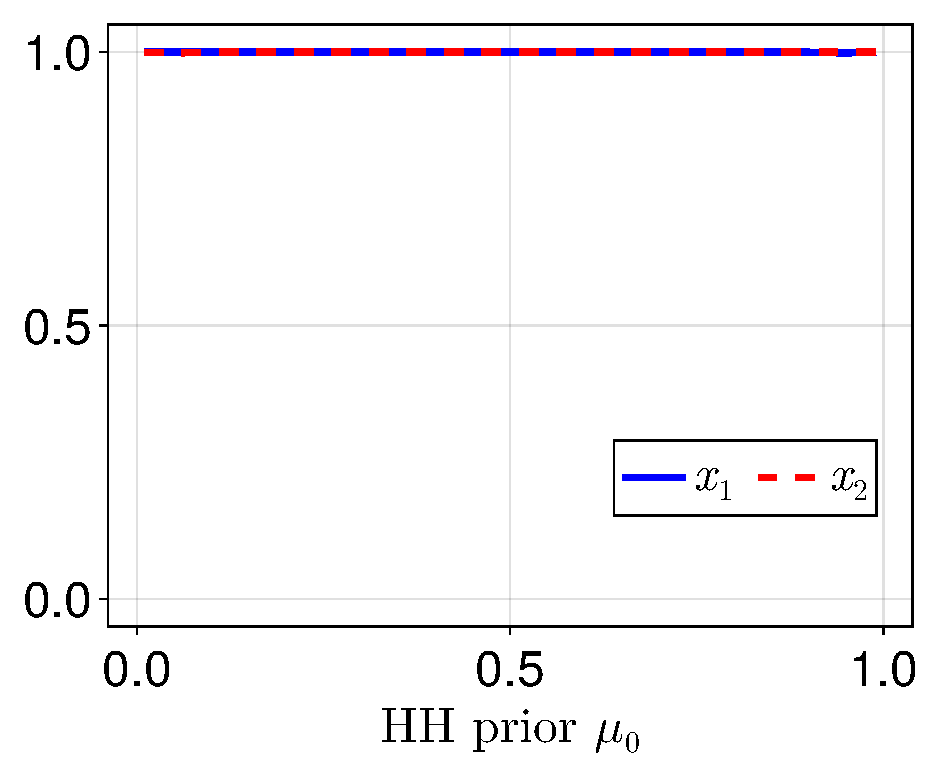
\includegraphics[width=0.49\textwidth]{figures/V8/γ_10/fig_optimal_π_across_μ_0_ω_1_1_ω_2_-1_δ_0.0_.pdf}
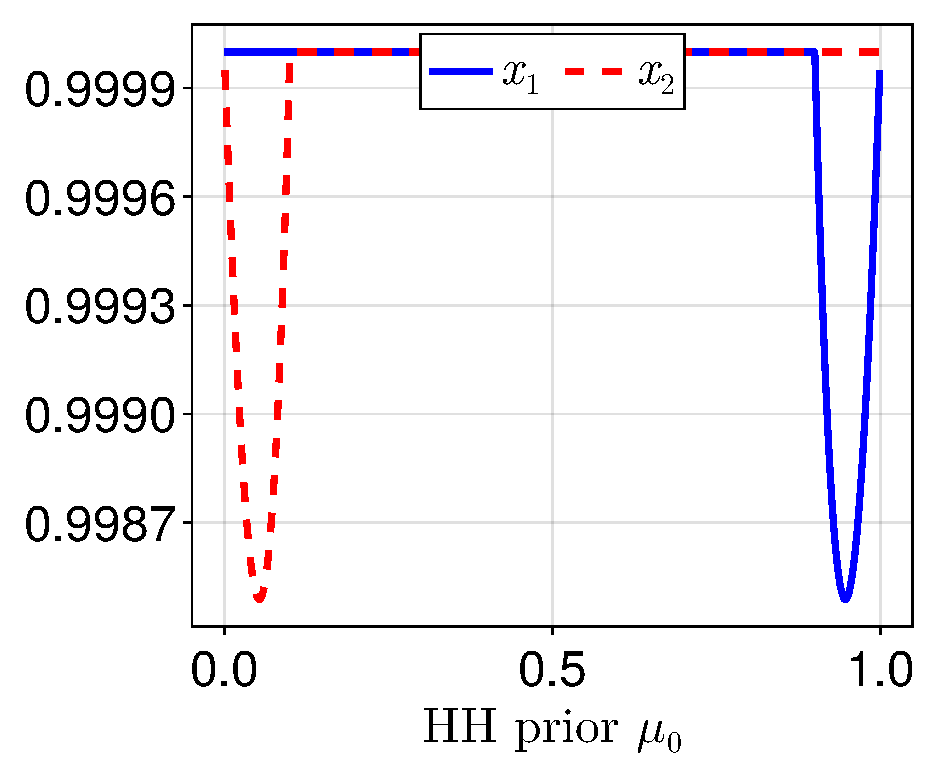
\includegraphics[width=0.49\textwidth]{figures/V11/γ=10.0-μ_0=0.5-α=1.0-θ=1.0-δ=0.0-ω_1=1.0-ω_2=-1.0/communication/fig_optimal_x_by_μ_0.pdf}
% 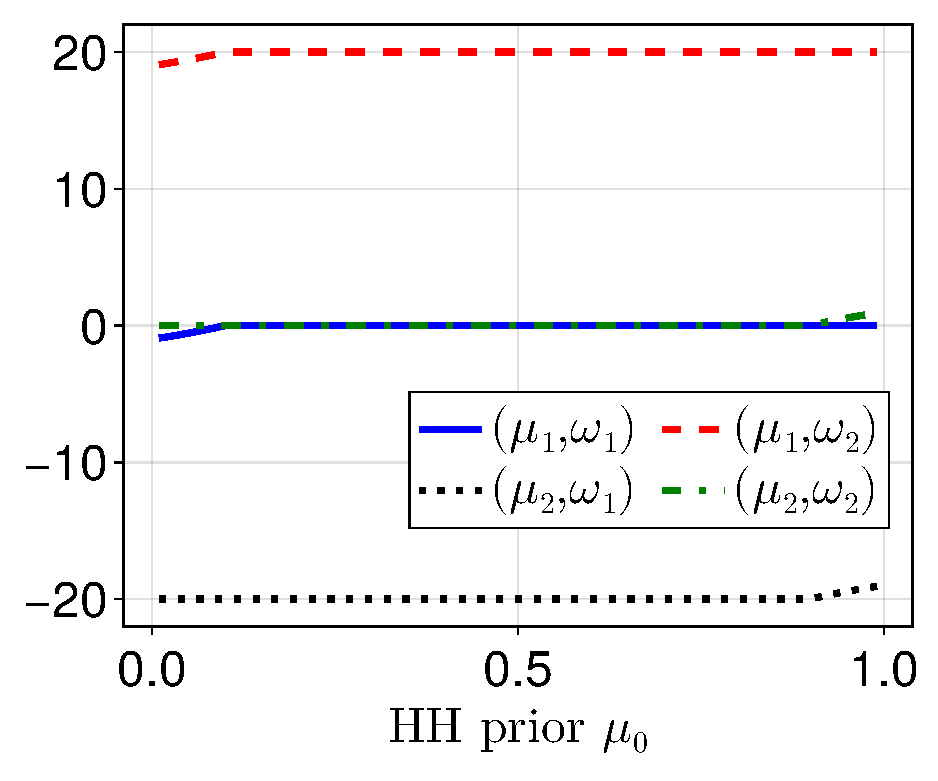
\includegraphics[width=0.49\textwidth]{figures/V8/γ_10/fig_posterior_across_μ_0_ω_1_1_ω_2_-1_δ_0.0_.pdf}
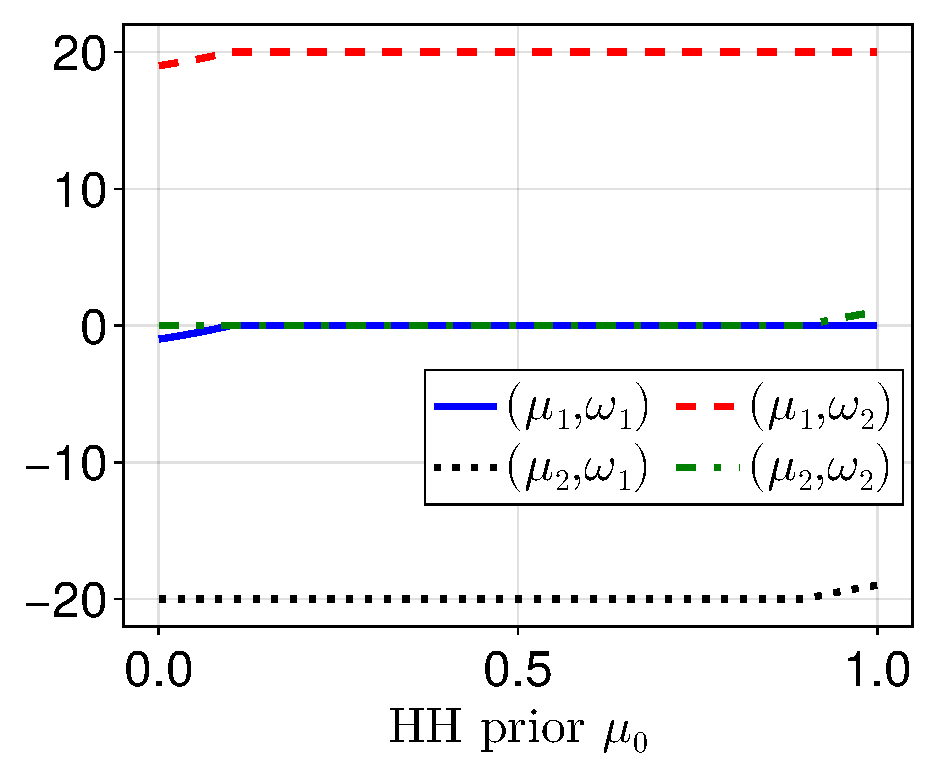
\includegraphics[width=0.49\textwidth]{figures/V11/γ=10.0-μ_0=0.5-α=1.0-θ=1.0-δ=0.0-ω_1=1.0-ω_2=-1.0/communication/fig_optimal_γ_by_μ_0.pdf}
\caption{Comparative statics for $\mu_0$, when $\delta=0$, holding fixed all other parameters as in the benchmark.}
\label{FigureA1}
\end{figure}

\begin{figure}[H]
\centering
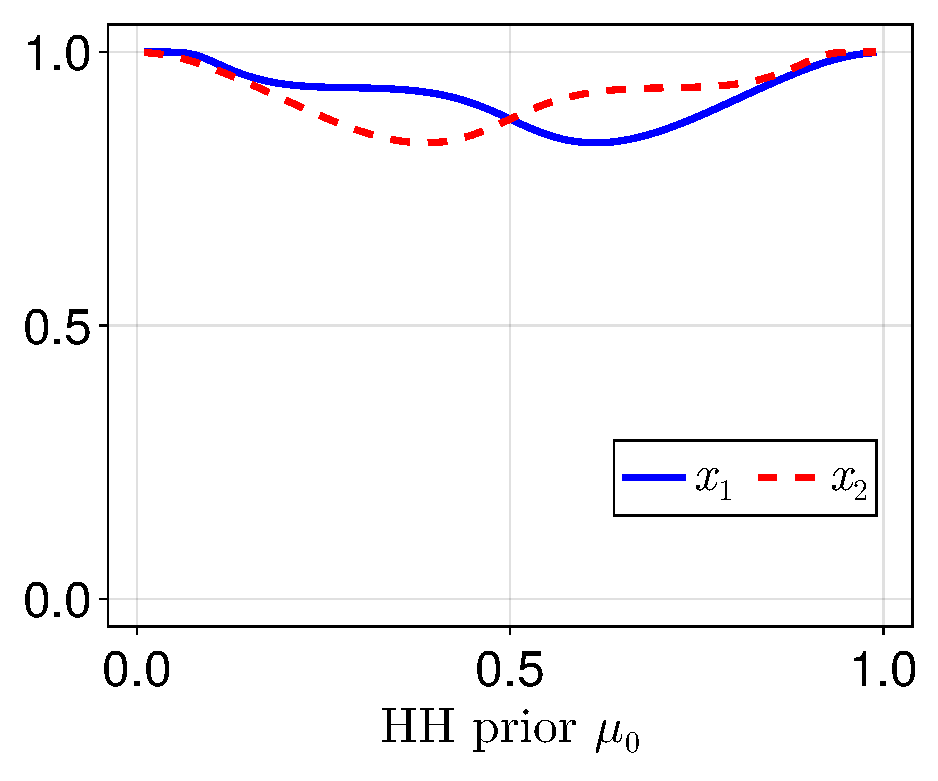
\includegraphics[width=0.49\textwidth]{figures/V8/γ_10/fig_optimal_π_across_μ_0_ω_1_1_ω_2_-1_δ_1.0_.pdf}
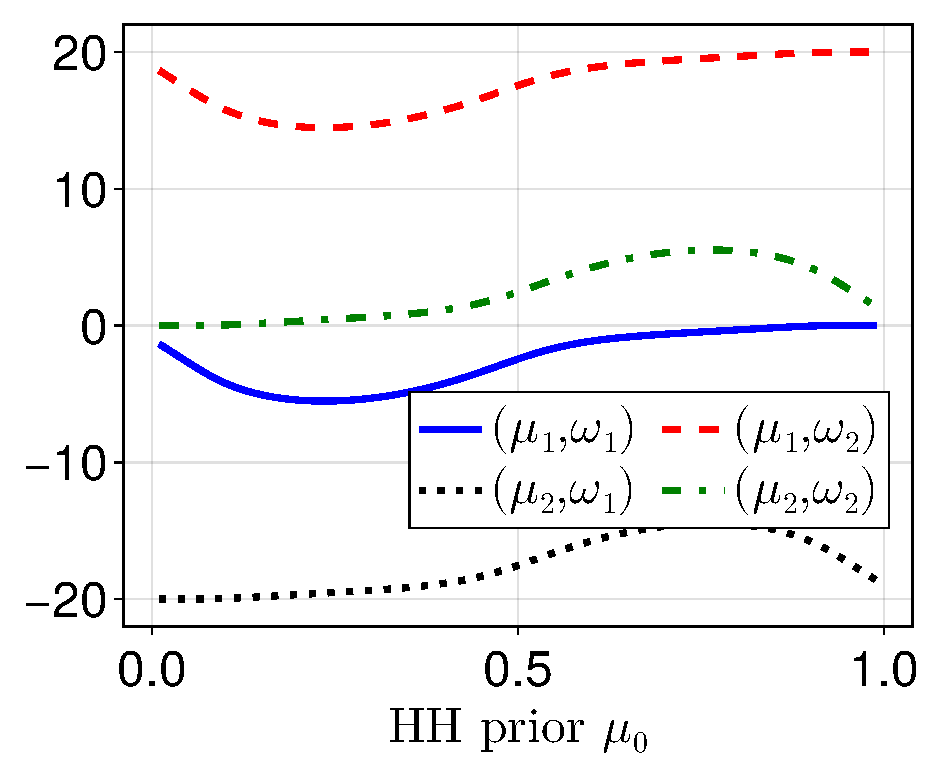
\includegraphics[width=0.49\textwidth]{figures/V8/γ_10/fig_posterior_across_μ_0_ω_1_1_ω_2_-1_δ_1.0_.pdf}
\caption{Comparative statics for $\mu_0$, when $\delta=1$, holding fixed all other parameters as in the benchmark.}
\label{FigureA2}
\end{figure}

\begin{figure}[H]
\centering
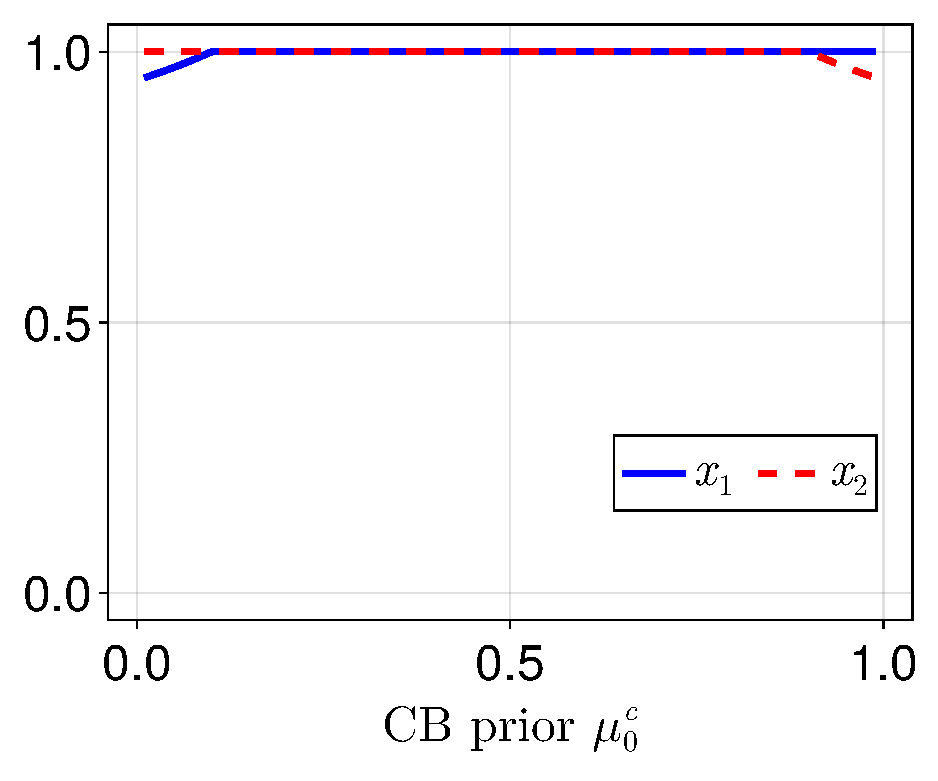
\includegraphics[width=0.49\textwidth]{figures/V8/γ_10/fig_optimal_π_across_μ_0_c_ω_1_1_ω_2_-1_δ_0.0_.pdf}
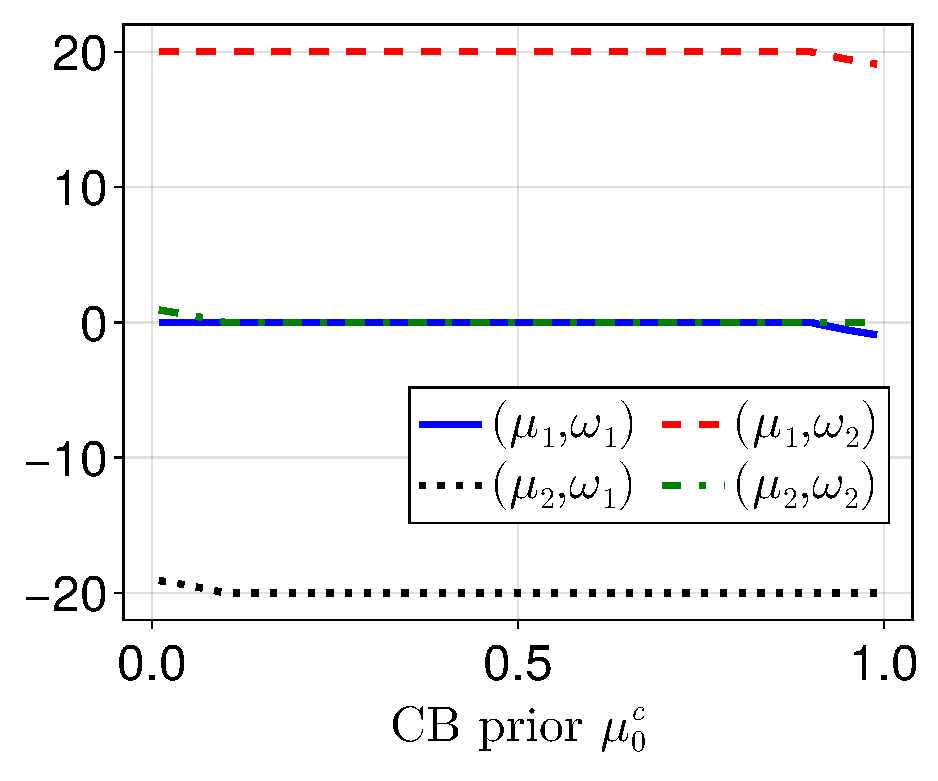
\includegraphics[width=0.49\textwidth]{figures/V8/γ_10/fig_posterior_across_μ_0_c_ω_1_1_ω_2_-1_δ_0.0_.pdf}
\caption{Comparative statics for $\mu_0^c$, when $\delta=0$, holding fixed all other parameters as in the benchmark.}
\label{FigureA3}
\end{figure}

\begin{figure}[H]
\centering
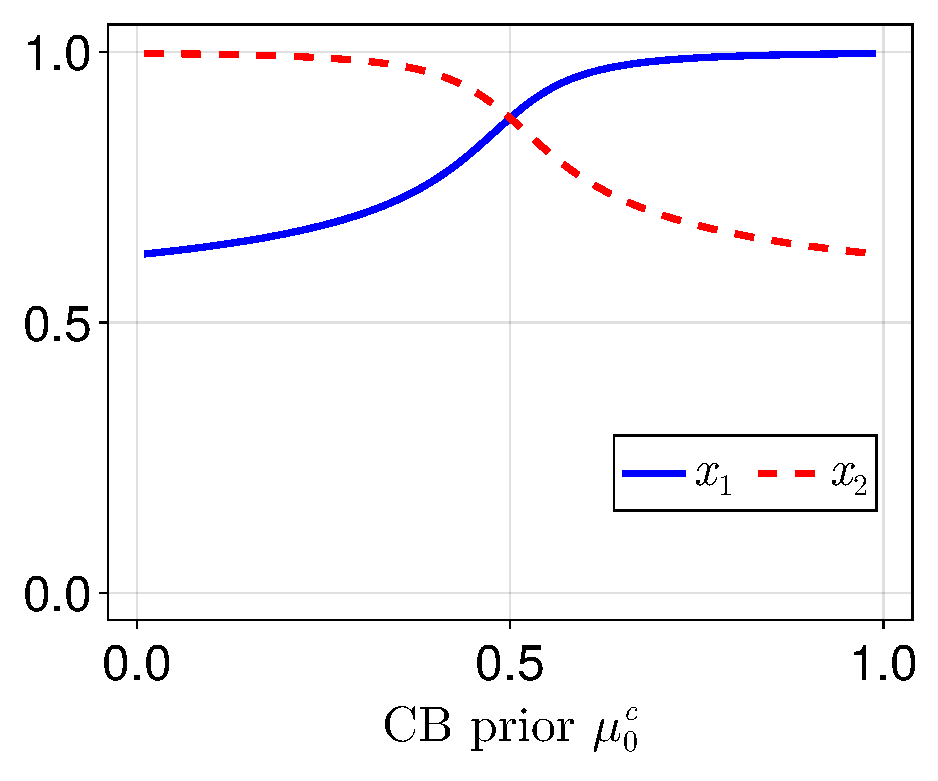
\includegraphics[width=0.49\textwidth]{figures/V8/γ_10/fig_optimal_π_across_μ_0_c_ω_1_1_ω_2_-1_δ_1.0_.pdf}
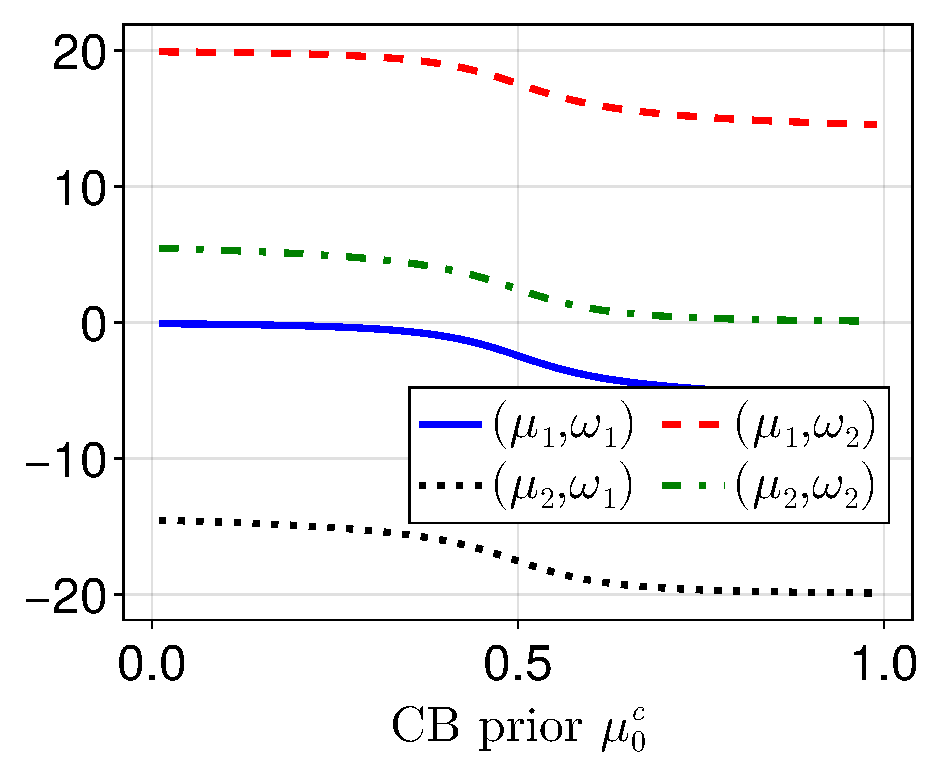
\includegraphics[width=0.49\textwidth]{figures/V8/γ_10/fig_posterior_across_μ_0_c_ω_1_1_ω_2_-1_δ_1.0_.pdf}
\caption{Comparative statics for $\mu_0^c$, when $\delta=1$, holding fixed all other parameters as in the benchmark.}
\label{FigureA4}
\end{figure}

\begin{figure}[H]
\centering
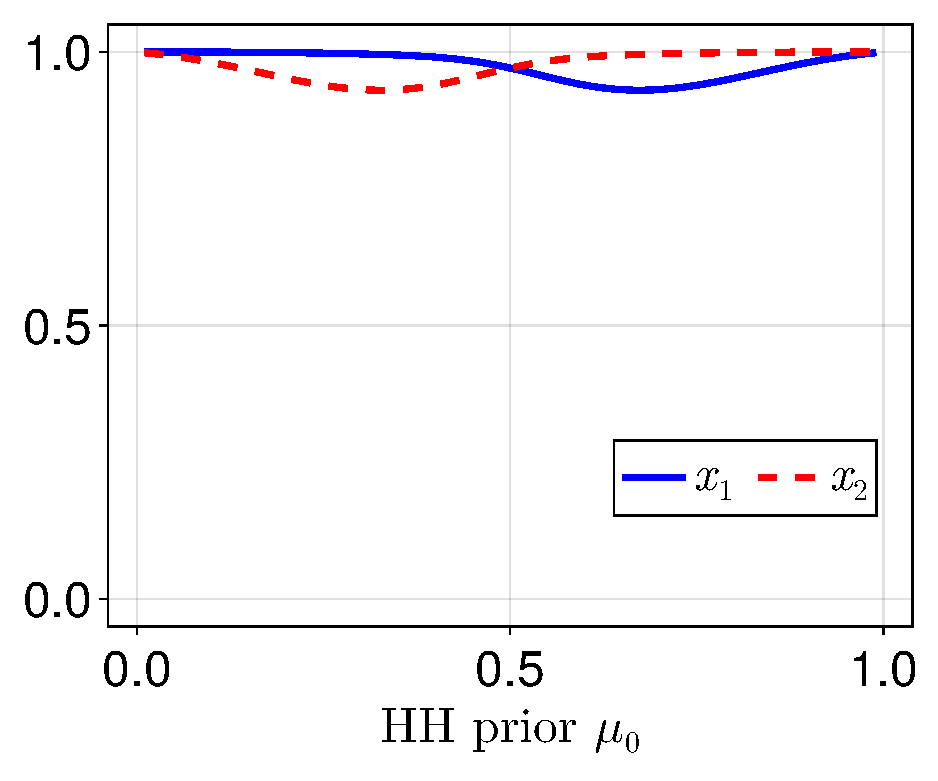
\includegraphics[width=0.49\textwidth]{figures/V8/γ_10/fig_optimal_π_across_μ_0_ω_1_2_ω_2_-2_δ_0.5_.pdf}
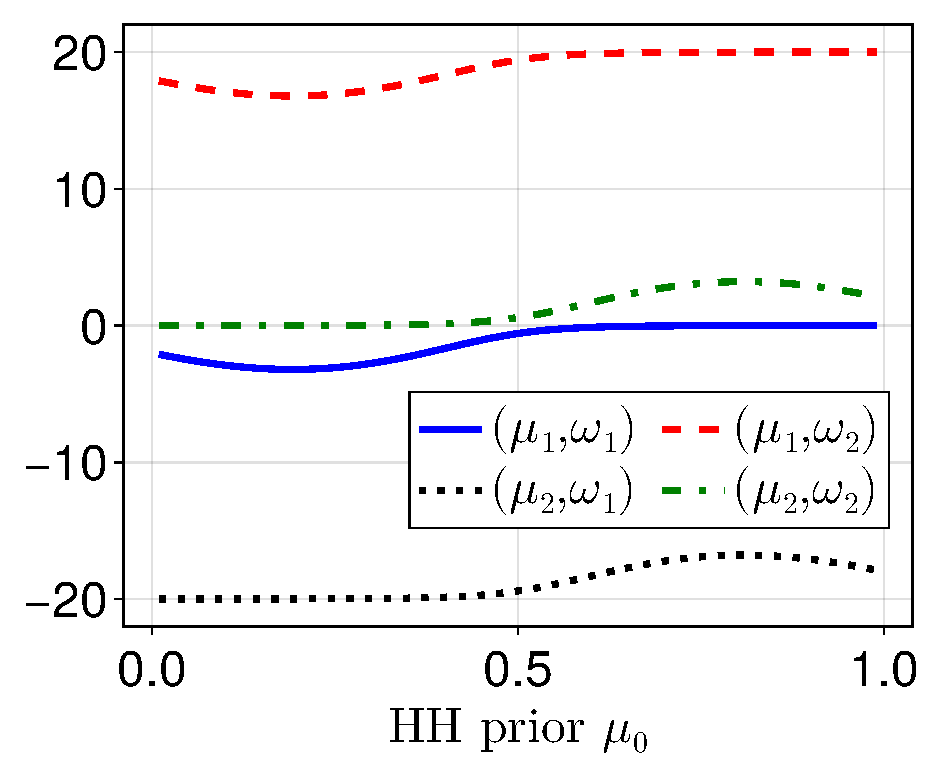
\includegraphics[width=0.49\textwidth]{figures/V8/γ_10/fig_posterior_across_μ_0_ω_1_2_ω_2_-2_δ_0.5_.pdf}
\caption{Comparative statics for $\mu_0$, when $(\omega_1,\omega_2)=(2,-2)$, holding fixed all other parameters as in the benchmark.}
\label{FigureA5}
\end{figure}

\begin{figure}[H]
\centering
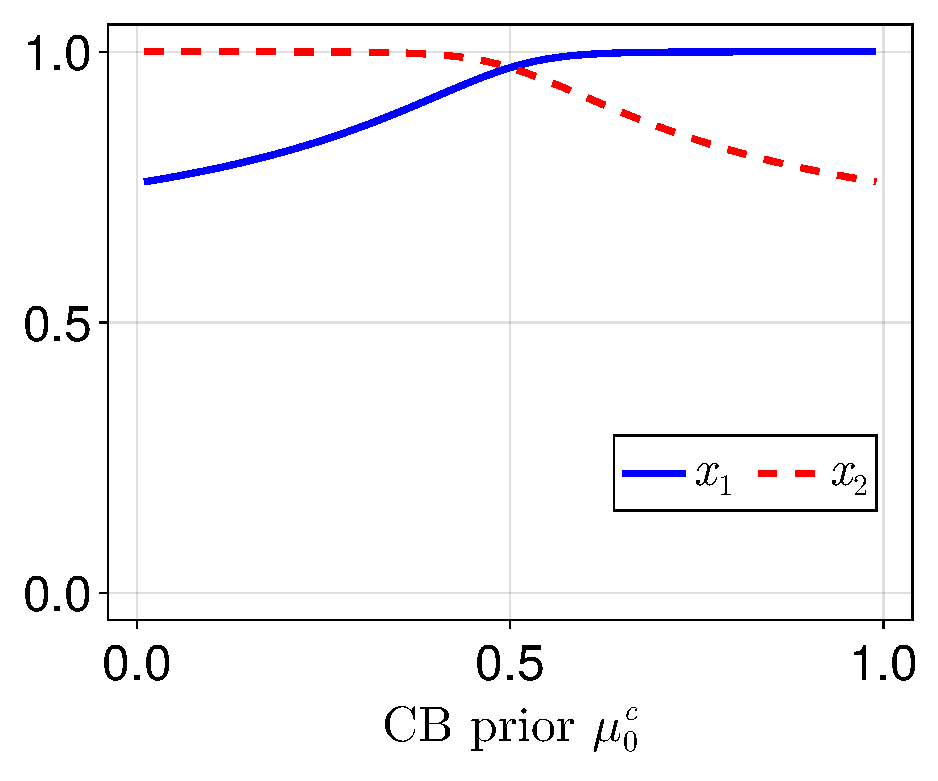
\includegraphics[width=0.49\textwidth]{figures/V8/γ_10/fig_optimal_π_across_μ_0_c_ω_1_2_ω_2_-2_δ_0.5_.pdf}
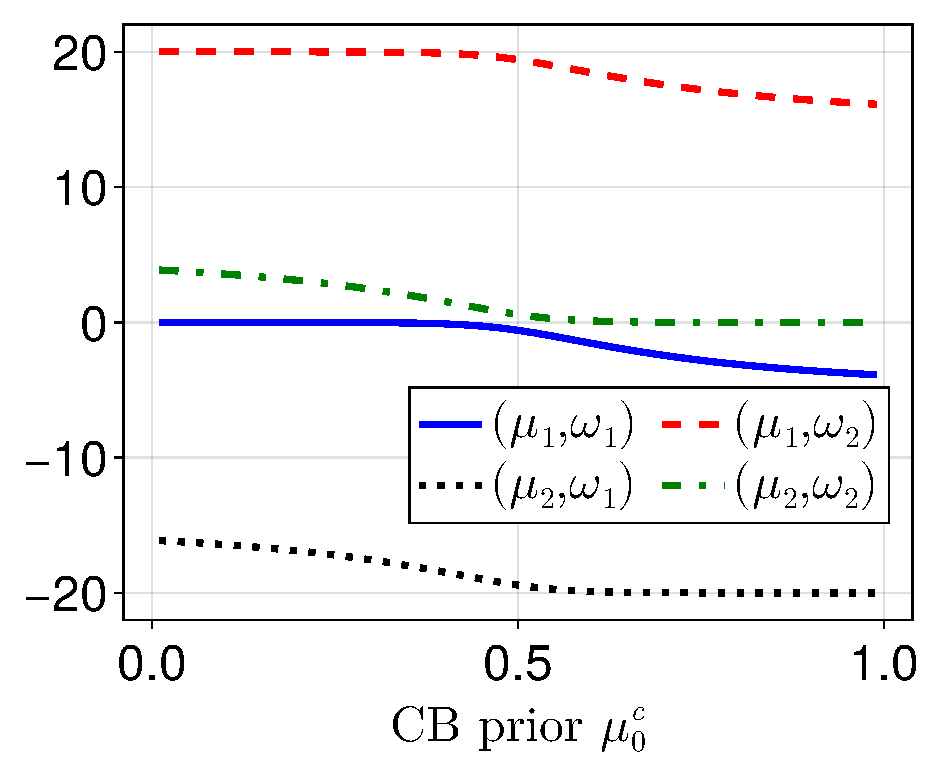
\includegraphics[width=0.49\textwidth]{figures/V8/γ_10/fig_posterior_across_μ_0_c_ω_1_2_ω_2_-2_δ_0.5_.pdf}
\caption{Comparative statics for $\mu_0^c$, when $(\omega_1,\omega_2)=(2,-2)$, holding fixed all other parameters as in the benchmark.}
\label{FigureA6}
\end{figure}

\begin{figure}[H]
\centering
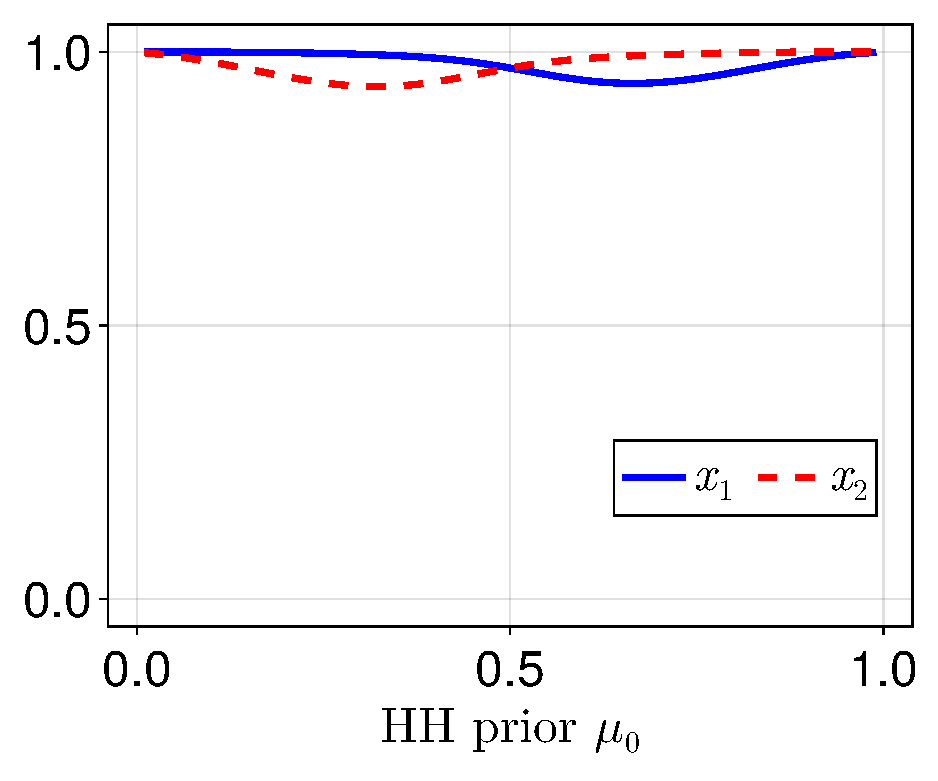
\includegraphics[width=0.49\textwidth]{figures/V8/γ_10/fig_optimal_π_across_μ_0_ω_1_2_ω_2_-1_δ_0.5_.pdf}
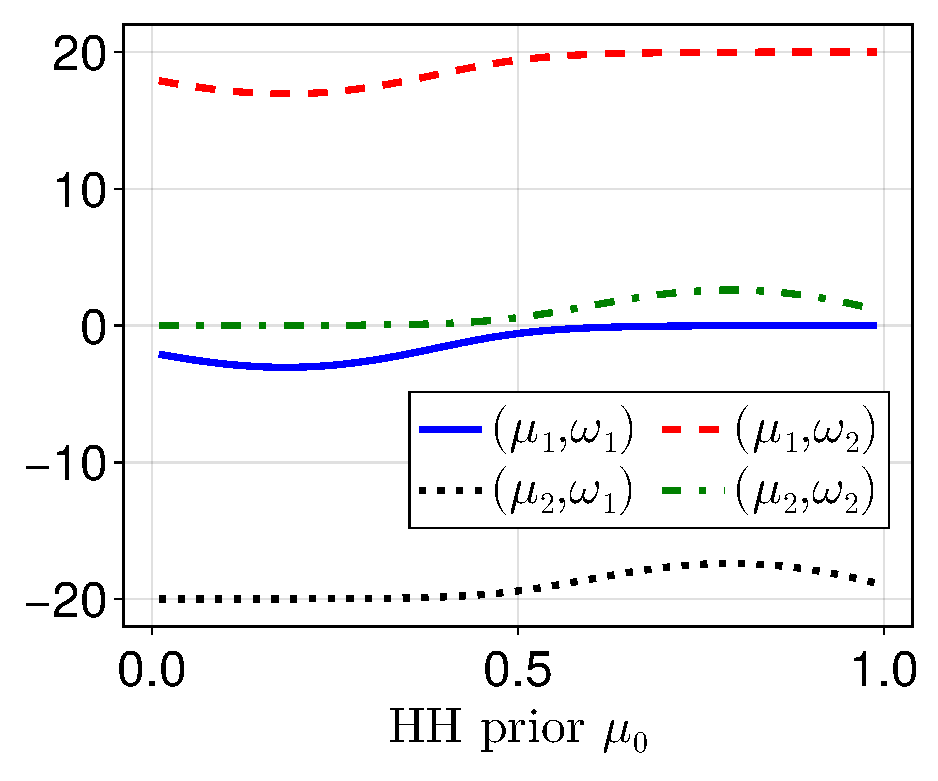
\includegraphics[width=0.49\textwidth]{figures/V8/γ_10/fig_posterior_across_μ_0_ω_1_2_ω_2_-1_δ_0.5_.pdf}
\caption{Comparative statics for $\mu_0$, when $(\omega_1,\omega_2)=(2,-1)$, holding fixed all other parameters as in the benchmark.}
\label{FigureA7}
\end{figure}

\begin{figure}[H]
\centering
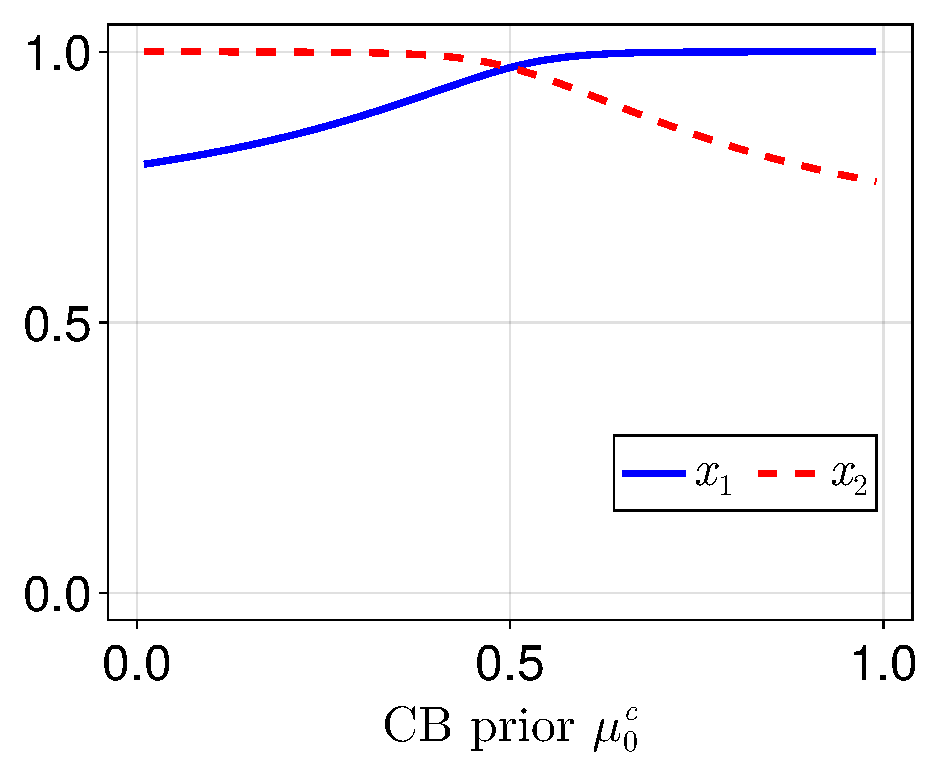
\includegraphics[width=0.49\textwidth]{figures/V8/γ_10/fig_optimal_π_across_μ_0_c_ω_1_2_ω_2_-1_δ_0.5_.pdf}
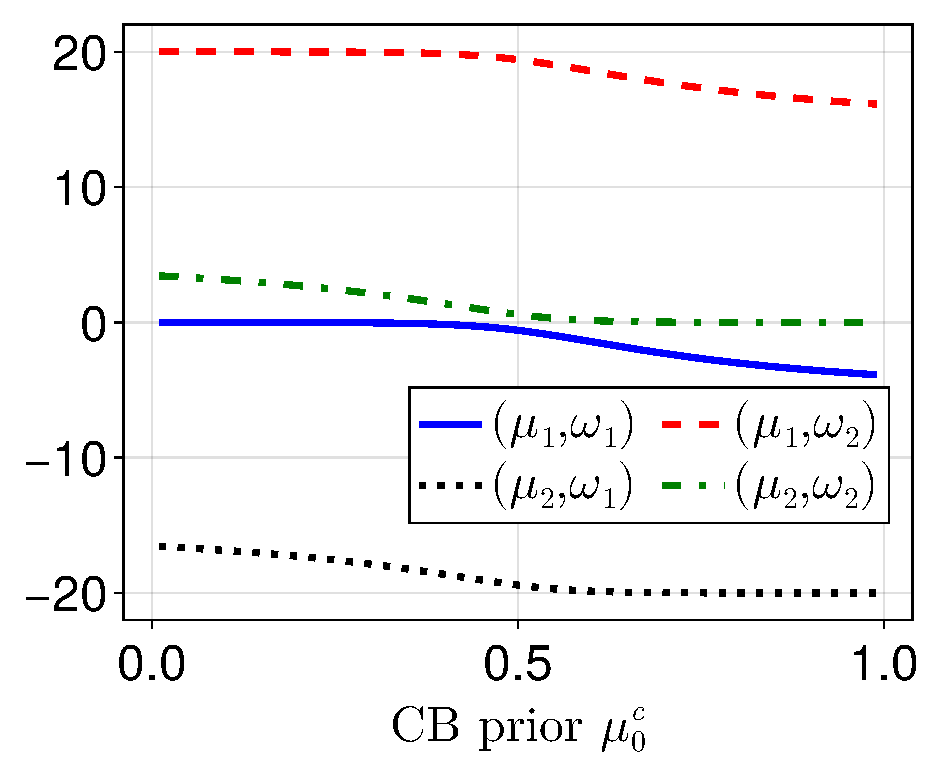
\includegraphics[width=0.49\textwidth]{figures/V8/γ_10/fig_posterior_across_μ_0_c_ω_1_2_ω_2_-1_δ_0.5_.pdf}
\caption{Comparative statics for $\mu_0^c$, when $(\omega_1,\omega_2)=(2,-1)$, holding fixed all other parameters as in the benchmark.}
\label{FigureA8}
\end{figure}

\begin{figure}[H]
\centering
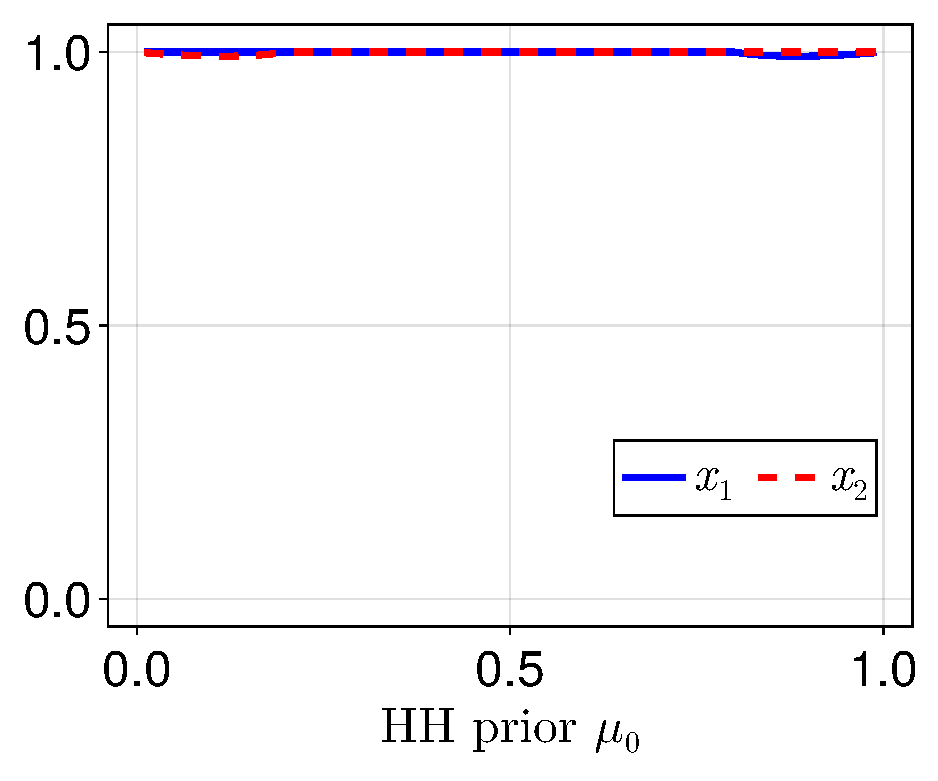
\includegraphics[width=0.49\textwidth]{figures/V8/γ_10/fig_optimal_π_across_μ_0_ω_1_2_ω_2_-2_δ_0.0_.pdf}
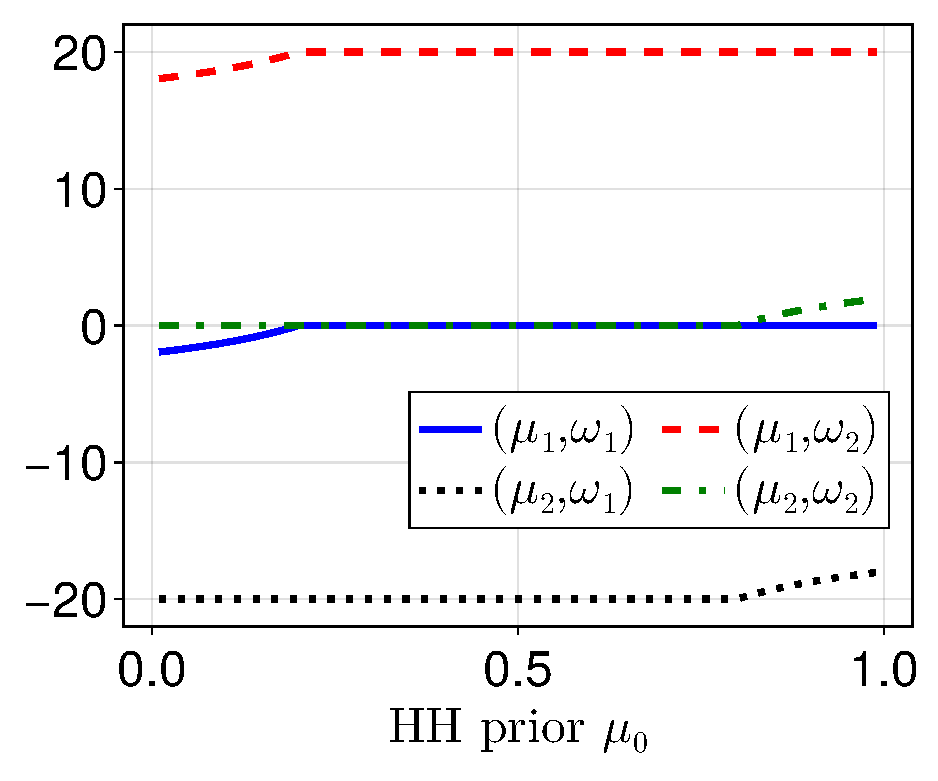
\includegraphics[width=0.49\textwidth]{figures/V8/γ_10/fig_posterior_across_μ_0_ω_1_2_ω_2_-2_δ_0.0_.pdf}
\caption{Comparative statics for $\mu_0$, when $(\delta,\omega_1,\omega_2)=(0,2,-2)$, holding fixed all other parameters as in the benchmark.}
\label{FigureA9}
\end{figure}

\begin{figure}[H]
\centering
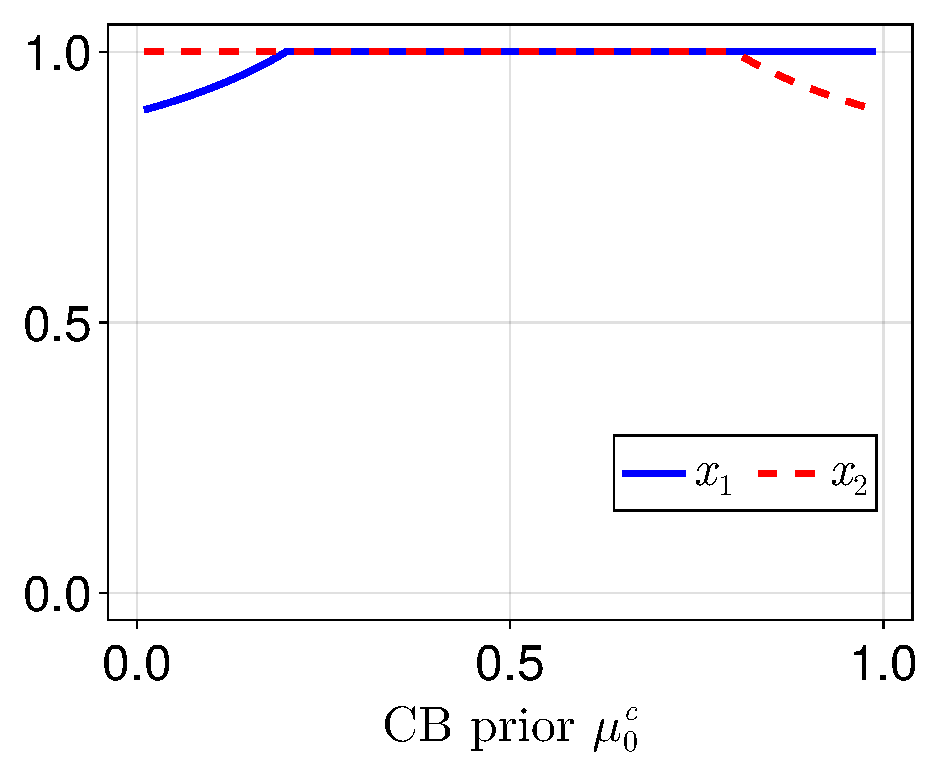
\includegraphics[width=0.49\textwidth]{figures/V8/γ_10/fig_optimal_π_across_μ_0_c_ω_1_2_ω_2_-2_δ_0.0_.pdf}
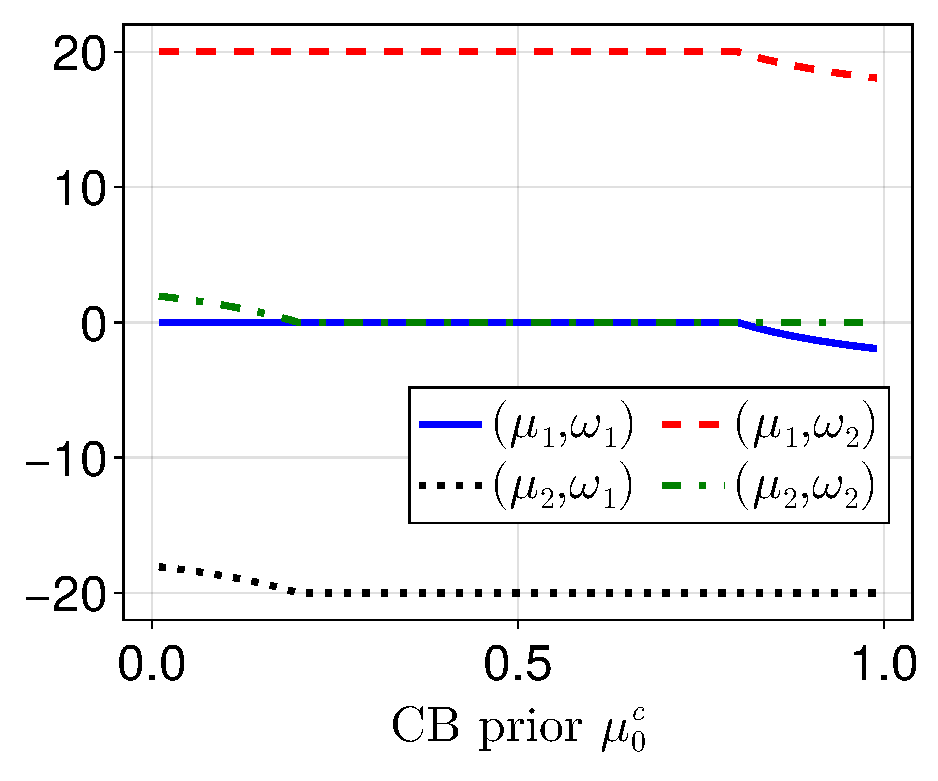
\includegraphics[width=0.49\textwidth]{figures/V8/γ_10/fig_posterior_across_μ_0_c_ω_1_2_ω_2_-2_δ_0.0_.pdf}
\caption{Comparative statics for $\mu_0^c$, when $(\delta,\omega_1,\omega_2)=(0,2,-2)$, holding fixed all other parameters as in the benchmark.}
\label{FigureA10}
\end{figure}

\begin{figure}[H]
\centering
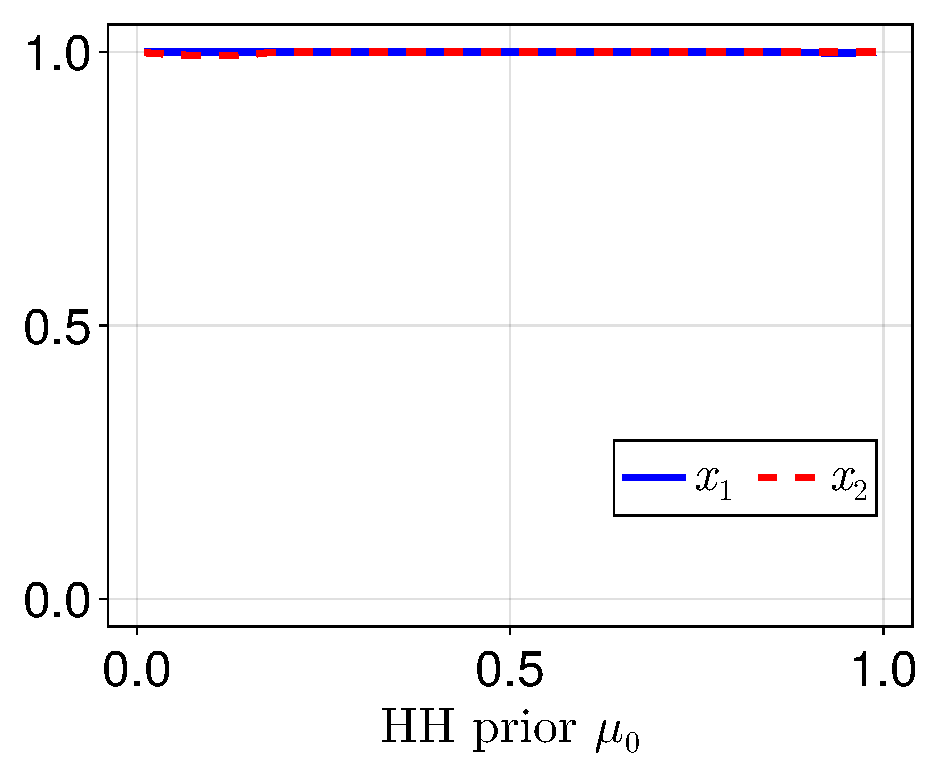
\includegraphics[width=0.49\textwidth]{figures/V8/γ_10/fig_optimal_π_across_μ_0_ω_1_2_ω_2_-1_δ_0.0_.pdf}
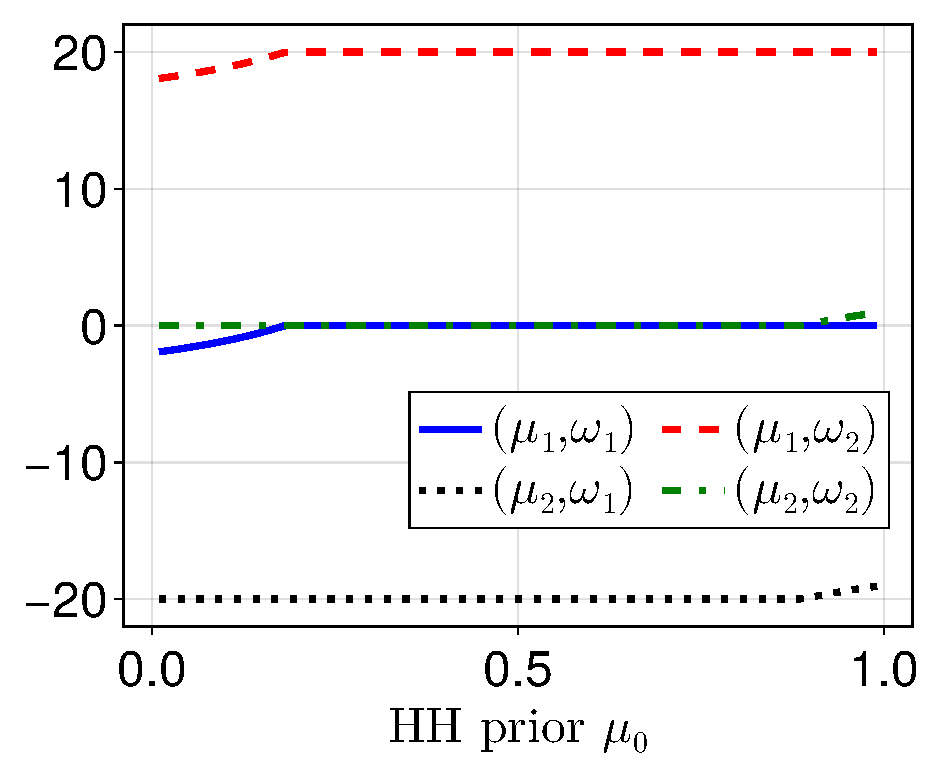
\includegraphics[width=0.49\textwidth]{figures/V8/γ_10/fig_posterior_across_μ_0_ω_1_2_ω_2_-1_δ_0.0_.pdf}
\caption{Comparative statics for $\mu_0$, when $(\delta,\omega_1,\omega_2)=(0,2,-1)$, holding fixed all other parameters as in the benchmark.}
\label{FigureA11}
\end{figure}

\begin{figure}[H]
\centering
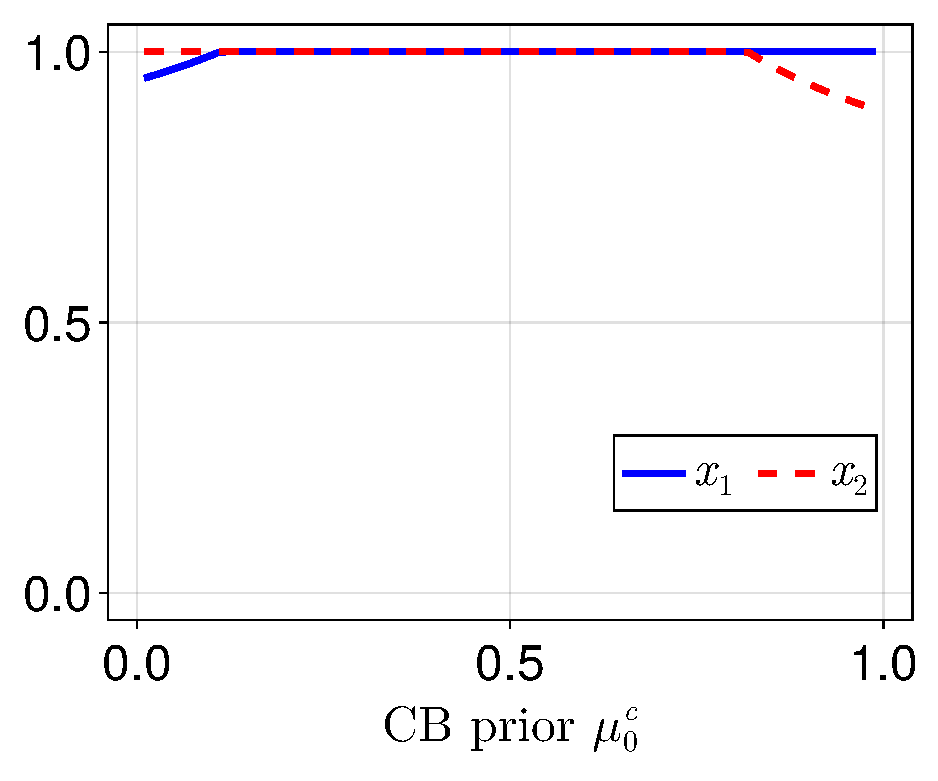
\includegraphics[width=0.49\textwidth]{figures/V8/γ_10/fig_optimal_π_across_μ_0_c_ω_1_2_ω_2_-1_δ_0.0_.pdf}
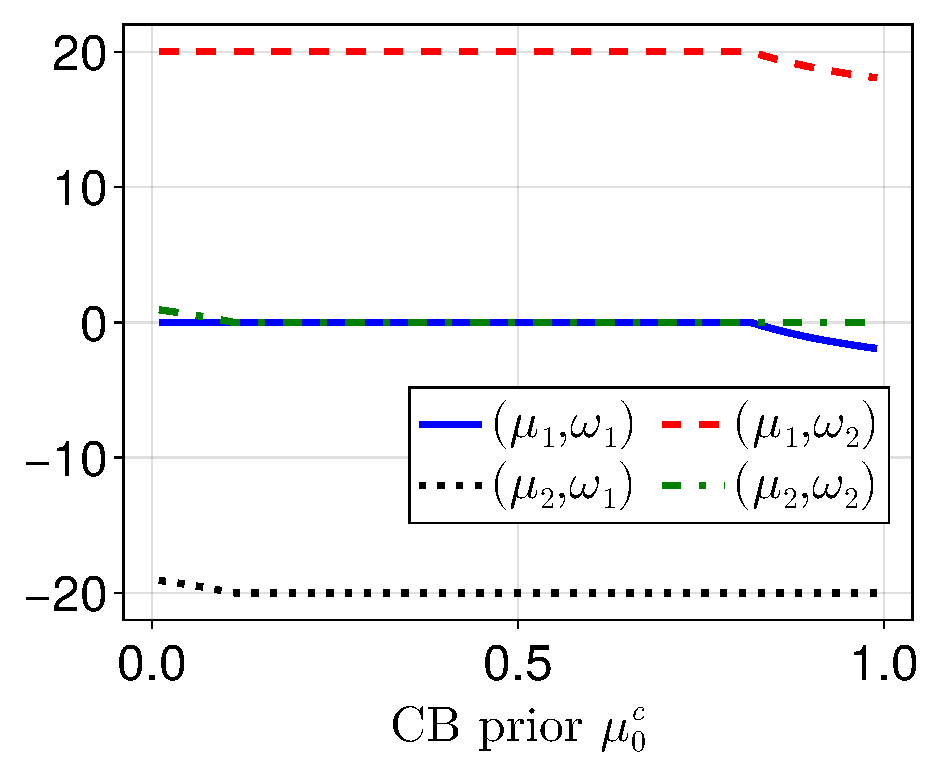
\includegraphics[width=0.49\textwidth]{figures/V8/γ_10/fig_posterior_across_μ_0_c_ω_1_2_ω_2_-1_δ_0.0_.pdf}
\caption{Comparative statics for $\mu_0^c$, when $(\delta,\omega_1,\omega_2)=(0,2,-1)$, holding fixed all other parameters as in the benchmark.}
\label{FigureA12}
\end{figure}

\begin{figure}[H]
\centering
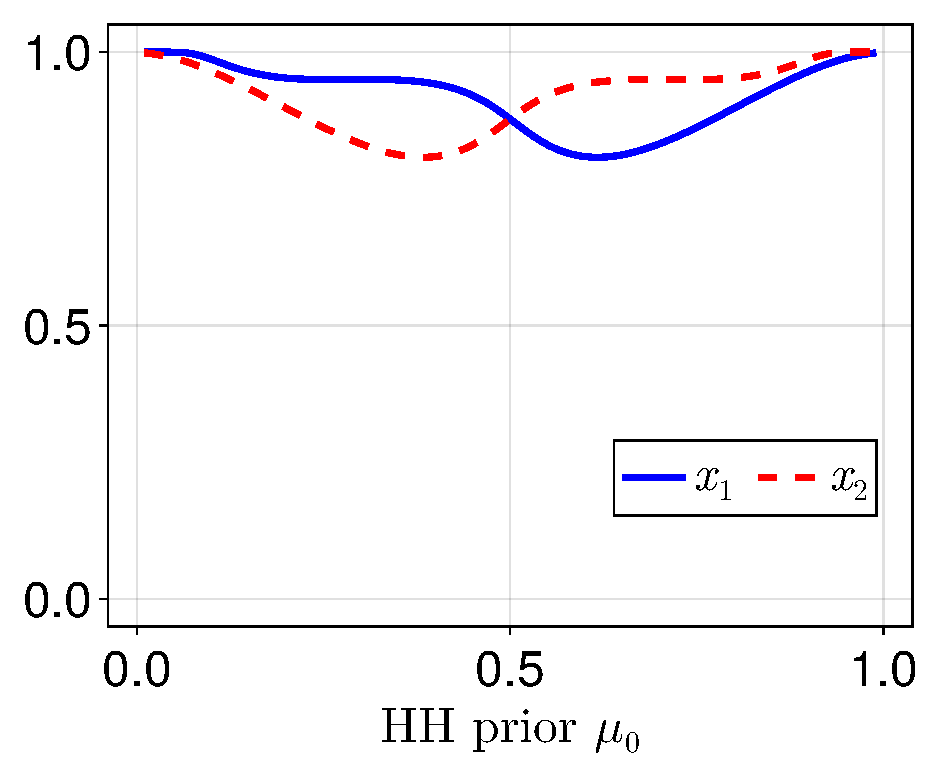
\includegraphics[width=0.49\textwidth]{figures/V8/γ_10/fig_optimal_π_across_μ_0_ω_1_2_ω_2_-2_δ_1.0_.pdf}
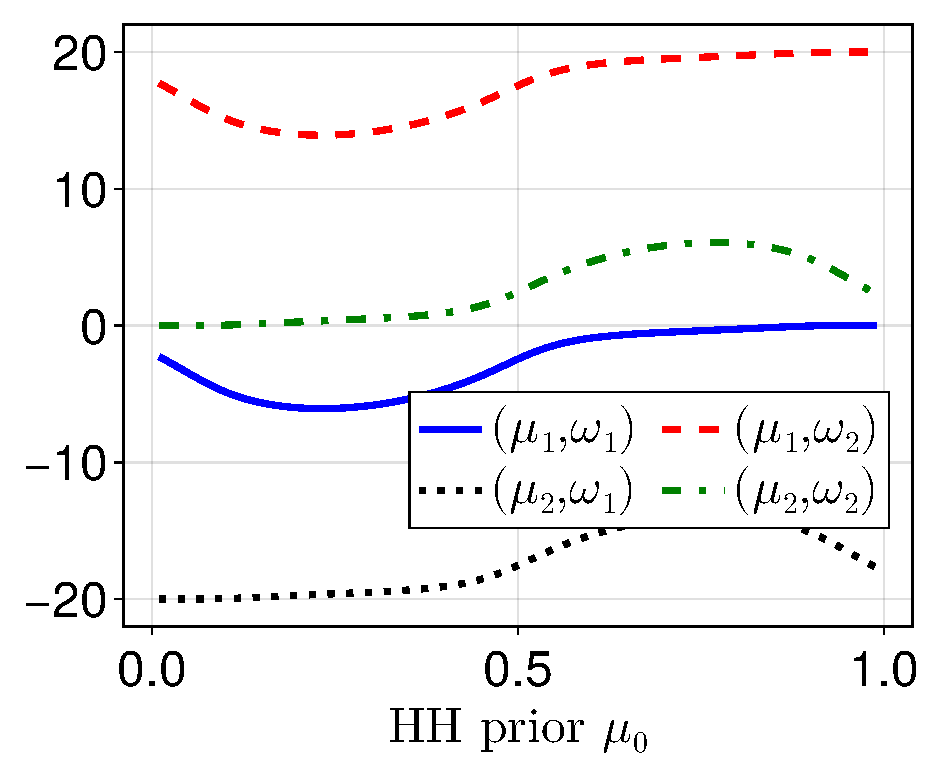
\includegraphics[width=0.49\textwidth]{figures/V8/γ_10/fig_posterior_across_μ_0_ω_1_2_ω_2_-2_δ_1.0_.pdf}
\caption{Comparative statics for $\mu_0$, when $(\delta,\omega_1,\omega_2)=(1,2,-2)$, holding fixed all other parameters as in the benchmark.}
\label{FigureA13}
\end{figure}

\begin{figure}[H]
\centering
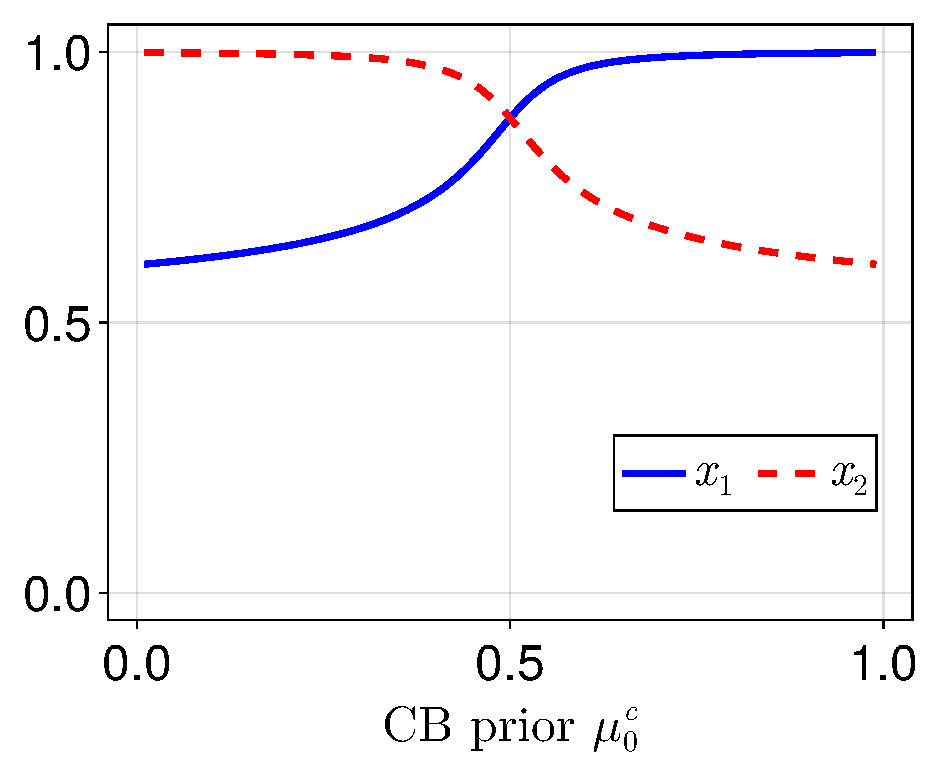
\includegraphics[width=0.49\textwidth]{figures/V8/γ_10/fig_optimal_π_across_μ_0_c_ω_1_2_ω_2_-2_δ_1.0_.pdf}
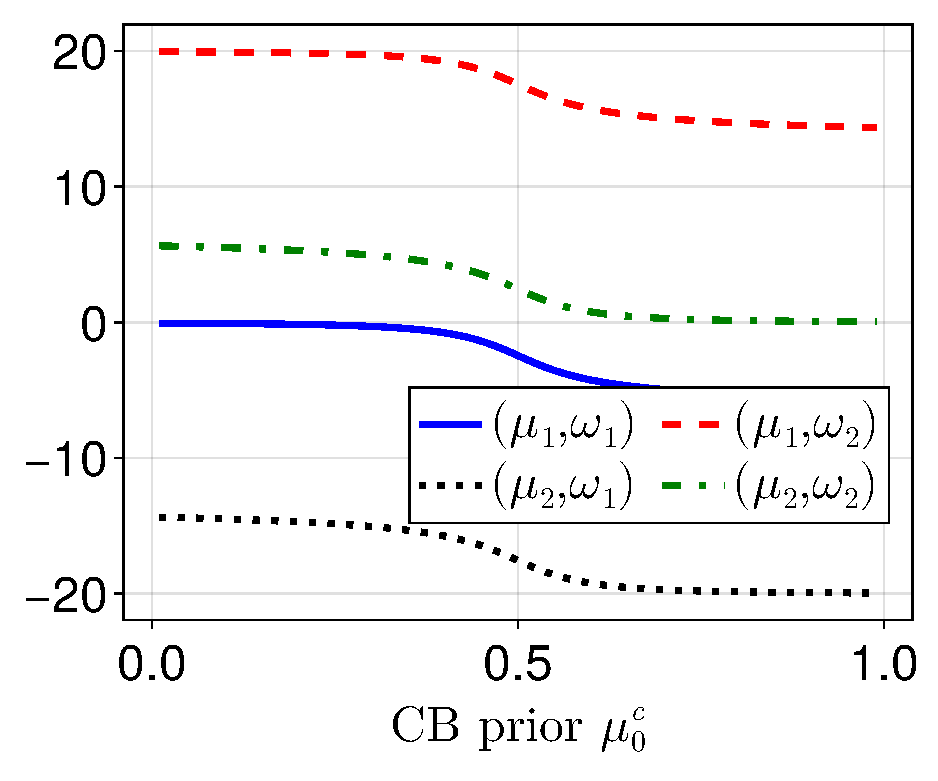
\includegraphics[width=0.49\textwidth]{figures/V8/γ_10/fig_posterior_across_μ_0_c_ω_1_2_ω_2_-2_δ_1.0_.pdf}
\caption{Comparative statics for $\mu_0^c$, when $(\delta,\omega_1,\omega_2)=(1,2,-2)$, holding fixed all other parameters as in the benchmark.}
\label{FigureA14}
\end{figure}

\begin{figure}[H]
\centering
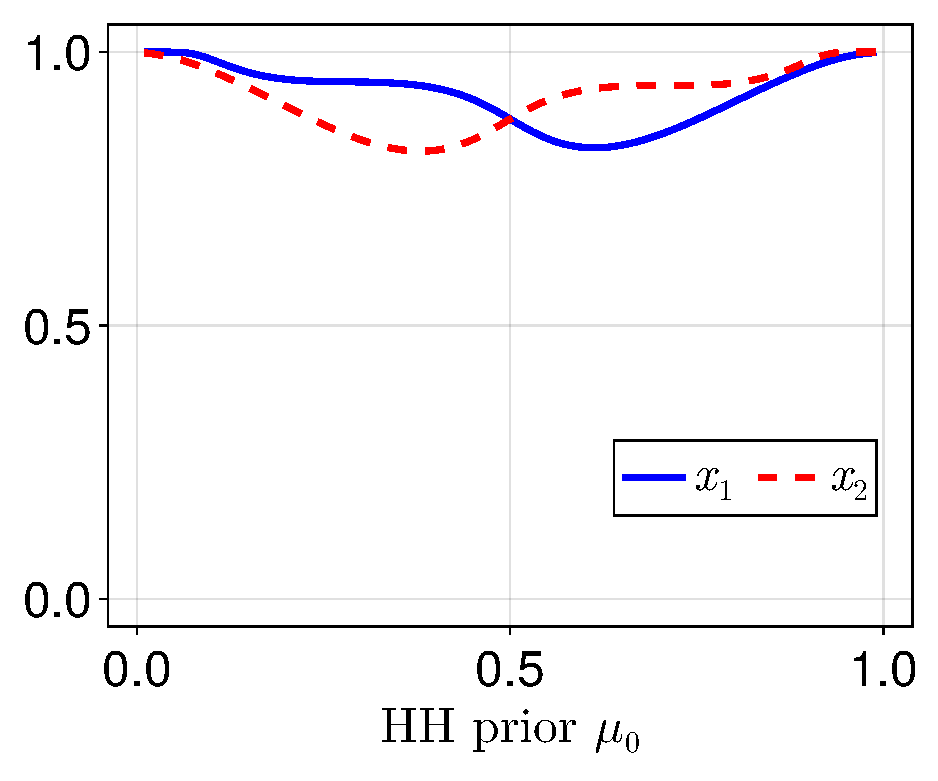
\includegraphics[width=0.49\textwidth]{figures/V8/γ_10/fig_optimal_π_across_μ_0_ω_1_2_ω_2_-1_δ_1.0_.pdf}
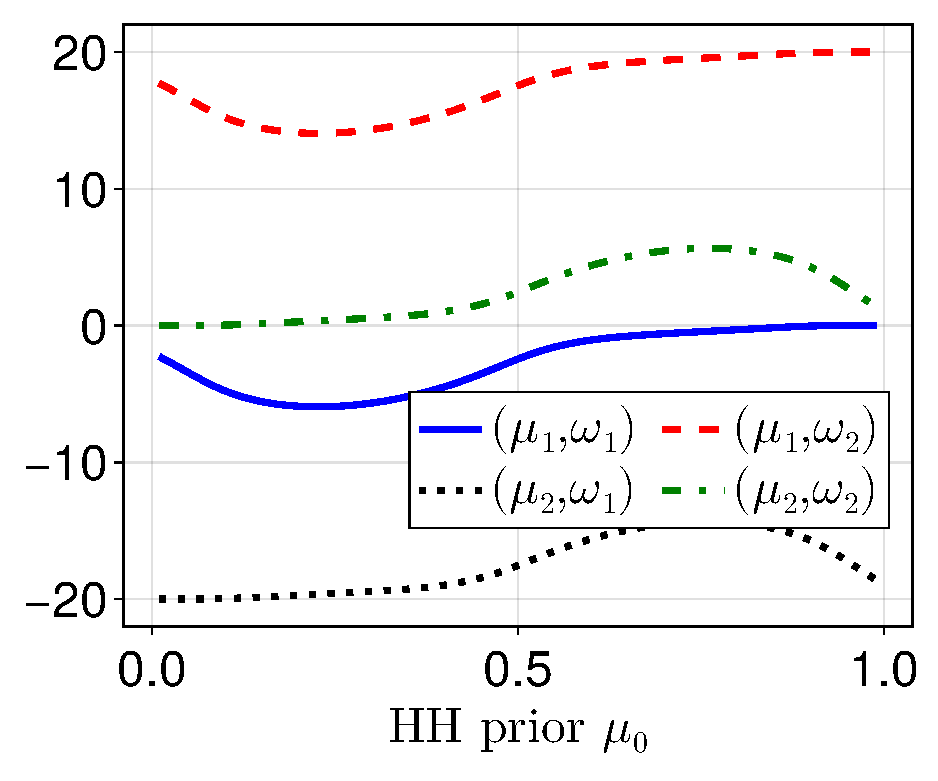
\includegraphics[width=0.49\textwidth]{figures/V8/γ_10/fig_posterior_across_μ_0_ω_1_2_ω_2_-1_δ_1.0_.pdf}
\caption{Comparative statics for $\mu_0$, when $(\delta,\omega_1,\omega_2)=(1,2,-1)$, holding fixed all other parameters as in the benchmark.}
\label{FigureA15}
\end{figure}

\begin{figure}[H]
\centering
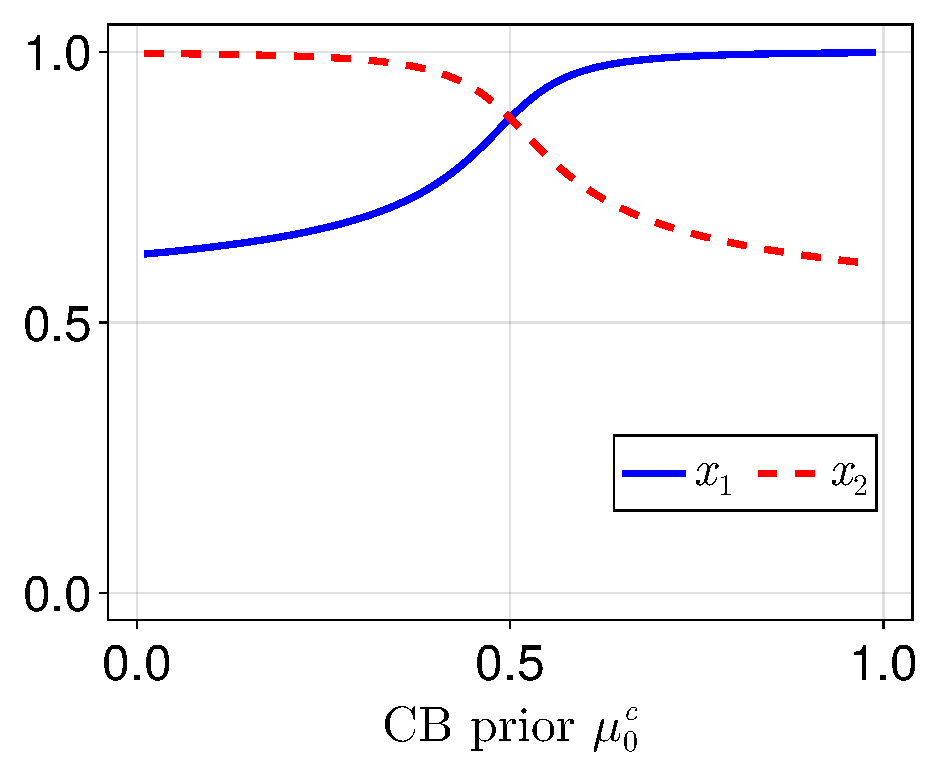
\includegraphics[width=0.49\textwidth]{figures/V8/γ_10/fig_optimal_π_across_μ_0_c_ω_1_2_ω_2_-1_δ_1.0_.pdf}
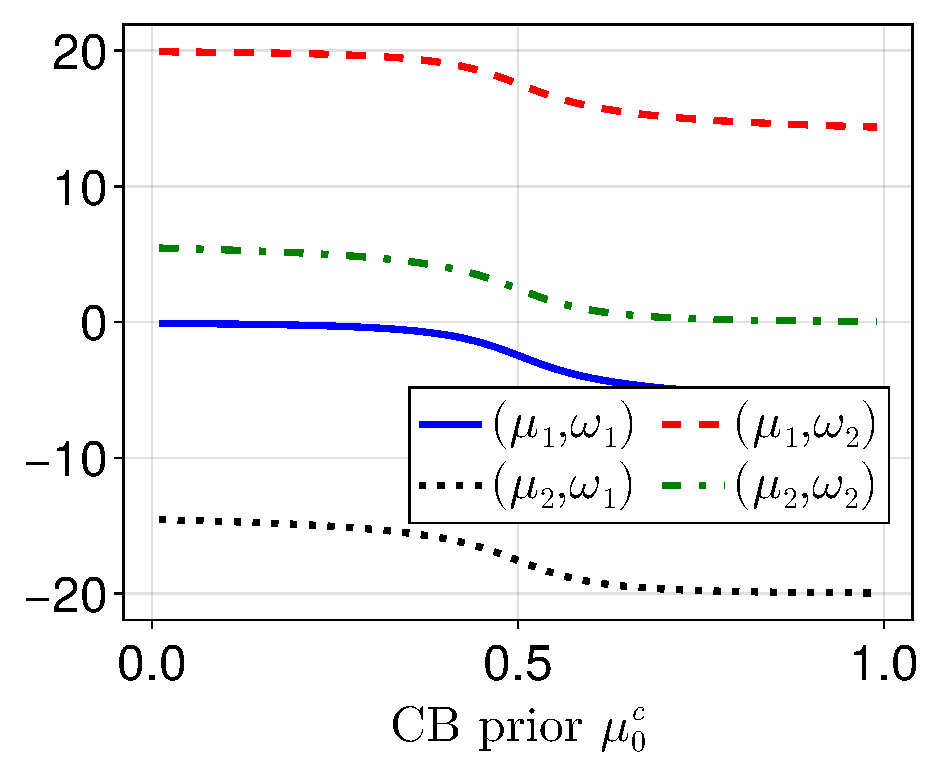
\includegraphics[width=0.49\textwidth]{figures/V8/γ_10/fig_posterior_across_μ_0_c_ω_1_2_ω_2_-1_δ_1.0_.pdf}
\caption{Comparative statics for $\mu_0^c$, when $(\delta,\omega_1,\omega_2)=(1,2,-1)$, holding fixed all other parameters as in the benchmark.}
\label{FigureA16}
\end{figure}

\begin{figure}[H]
\centering
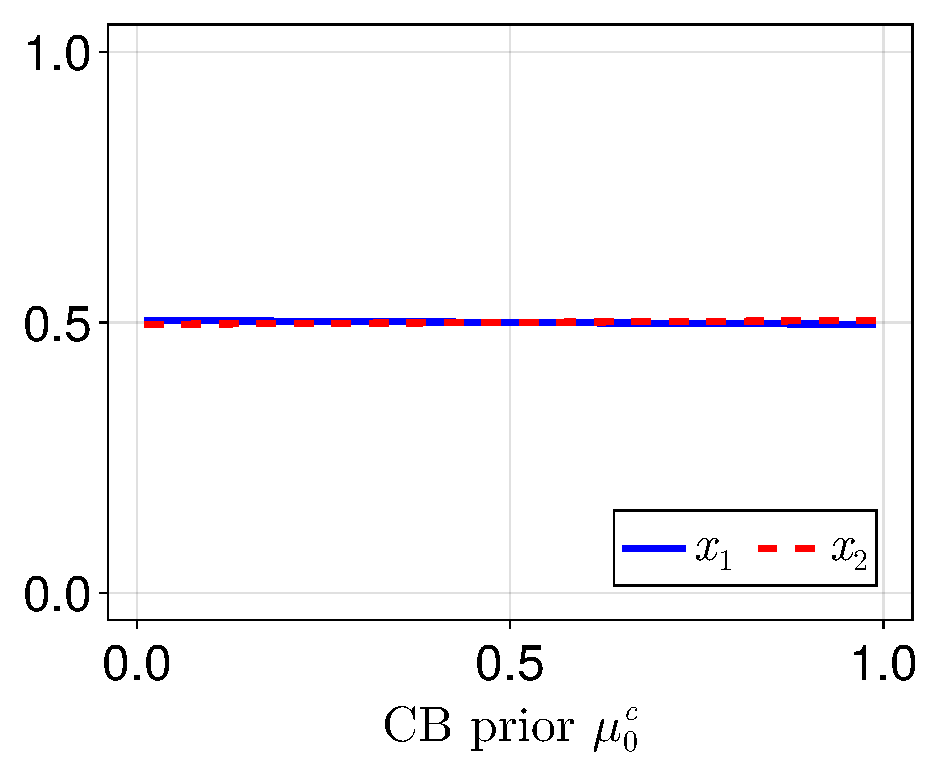
\includegraphics[width=0.49\textwidth]{figures/V8/γ_1/fig_optimal_π_across_μ_0_c_ω_1_1_ω_2_-1_δ_0.5_.pdf}
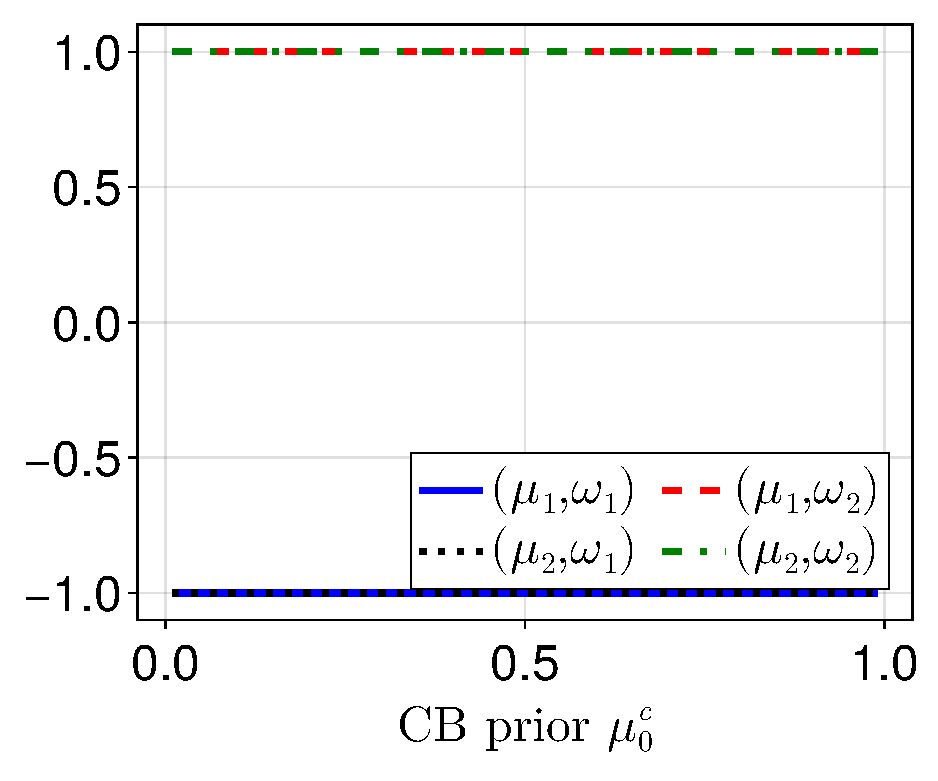
\includegraphics[width=0.49\textwidth]{figures/V8/γ_1/fig_posterior_across_μ_0_c_ω_1_1_ω_2_-1_δ_0.5_.pdf}
\caption{Comparative statics for $\mu_0^c$ varying from 0 to 1, holding fixed all other parameters as in the benchmark.}
\label{Figure4}
\end{figure}


\begin{figure}[H]
\centering
\includegraphics[width=0.49\textwidth]{figures/V8/γ_1/fig_optimal_π_across_μ_0_ω_1_2_ω_2_-2_δ_0.5_.pdf}
\includegraphics[width=0.49\textwidth]{figures/V8/γ_1/fig_posterior_across_μ_0_ω_1_2_ω_2_-2_δ_0.5_.pdf}
\caption{Comparative statics for $\mu_0$, when $(\omega_1,\omega_2)=(2,-2)$, holding fixed all other parameters as in the benchmark.}
\label{FigureA17}
\end{figure}


\begin{figure}[H]
\centering
\includegraphics[width=0.49\textwidth]{figures/V8/γ_1/fig_optimal_π_across_μ_0_c_ω_1_2_ω_2_-2_δ_0.5_.pdf}
\includegraphics[width=0.49\textwidth]{figures/V8/γ_1/fig_posterior_across_μ_0_c_ω_1_2_ω_2_-2_δ_0.5_.pdf}
\caption{Comparative statics for $\mu_0^c$, when $(\omega_1,\omega_2)=(2,-2)$, holding fixed all other parameters as in the benchmark.}
\label{FigureA18}
\end{figure}

\begin{figure}[H]
\centering
\includegraphics[width=0.49\textwidth]{figures/V8/γ_1/fig_optimal_π_across_μ_0_ω_1_2_ω_2_-1_δ_0.5_.pdf}
\includegraphics[width=0.49\textwidth]{figures/V8/γ_1/fig_posterior_across_μ_0_ω_1_2_ω_2_-1_δ_0.5_.pdf}
\caption{Comparative statics for $\mu_0$, when $(\omega_1,\omega_2)=(2,-1)$, holding fixed all other parameters as in the benchmark.}
\label{FigureA19}
\end{figure}

\begin{figure}[H]
\centering
\includegraphics[width=0.49\textwidth]{figures/V8/γ_1/fig_optimal_π_across_μ_0_c_ω_1_2_ω_2_-1_δ_0.5_.pdf}
\includegraphics[width=0.49\textwidth]{figures/V8/γ_1/fig_posterior_across_μ_0_c_ω_1_2_ω_2_-1_δ_0.5_.pdf}
\caption{Comparative statics for $\mu_0^c$, when $(\omega_1,\omega_2)=(2,-1)$, holding fixed all other parameters as in the benchmark.}
\label{FigureA20}
\end{figure}

\begin{figure}[H]
\centering
\includegraphics[width=0.49\textwidth]{figures/V8/γ_1/fig_optimal_π_across_μ_0_ω_1_1_ω_2_-1_δ_0.0_.pdf}
\includegraphics[width=0.49\textwidth]{figures/V8/γ_1/fig_posterior_across_μ_0_ω_1_1_ω_2_-1_δ_0.0_.pdf}
\caption{Comparative statics for $\mu_0$, when $\delta=0$, holding fixed all other parameters as in the benchmark.}
\label{FigureA21}
\end{figure}

\begin{figure}[H]
\centering
\includegraphics[width=0.49\textwidth]{figures/V8/γ_1/fig_optimal_π_across_μ_0_c_ω_1_1_ω_2_-1_δ_0.0_.pdf}
\includegraphics[width=0.49\textwidth]{figures/V8/γ_1/fig_posterior_across_μ_0_c_ω_1_1_ω_2_-1_δ_0.0_.pdf}
\caption{Comparative statics for $\mu_0^c$, when $\delta=0$, holding fixed all other parameters as in the benchmark.}
\label{FigureA22}
\end{figure}

\begin{figure}[H]
\centering
\includegraphics[width=0.49\textwidth]{figures/V8/γ_1/fig_optimal_π_across_μ_0_ω_1_1_ω_2_-1_δ_1.0_.pdf}
\includegraphics[width=0.49\textwidth]{figures/V8/γ_1/fig_posterior_across_μ_0_ω_1_1_ω_2_-1_δ_1.0_.pdf}
\caption{Comparative statics for $\mu_0$, when $\delta=1$, holding fixed all other parameters as in the benchmark.}
\label{FigureA23}
\end{figure}

\begin{figure}[H]
\centering
\includegraphics[width=0.49\textwidth]{figures/V8/γ_1/fig_optimal_π_across_μ_0_c_ω_1_1_ω_2_-1_δ_1.0_.pdf}
\includegraphics[width=0.49\textwidth]{figures/V8/γ_1/fig_posterior_across_μ_0_c_ω_1_1_ω_2_-1_δ_1.0_.pdf}
\caption{Comparative statics for $\mu_0^c$, when $\delta=1$, holding fixed all other parameters as in the benchmark.}
\label{FigureA24}
\end{figure}

\begin{figure}[H]
\centering
\includegraphics[width=0.49\textwidth]{figures/V8/γ_1/fig_optimal_π_across_μ_0_ω_1_2_ω_2_-2_δ_0.0_.pdf}
\includegraphics[width=0.49\textwidth]{figures/V8/γ_1/fig_posterior_across_μ_0_ω_1_2_ω_2_-2_δ_0.0_.pdf}
\caption{Comparative statics for $\mu_0$, when $(\delta,\omega_1,\omega_2)=(0,2,-2)$, holding fixed all other parameters as in the benchmark.}
\label{FigureA25}
\end{figure}

\begin{figure}[H]
\centering
\includegraphics[width=0.49\textwidth]{figures/V8/γ_1/fig_optimal_π_across_μ_0_c_ω_1_2_ω_2_-2_δ_0.0_.pdf}
\includegraphics[width=0.49\textwidth]{figures/V8/γ_1/fig_posterior_across_μ_0_c_ω_1_2_ω_2_-2_δ_0.0_.pdf}
\caption{Comparative statics for $\mu_0^c$, when $(\delta,\omega_1,\omega_2)=(0,2,-2)$, holding fixed all other parameters as in the benchmark.}
\label{FigureA26}
\end{figure}

\begin{figure}[H]
\centering
\includegraphics[width=0.49\textwidth]{figures/V8/γ_1/fig_optimal_π_across_μ_0_ω_1_2_ω_2_-1_δ_0.0_.pdf}
\includegraphics[width=0.49\textwidth]{figures/V8/γ_1/fig_posterior_across_μ_0_ω_1_2_ω_2_-1_δ_0.0_.pdf}
\caption{Comparative statics for $\mu_0$, when $(\delta,\omega_1,\omega_2)=(0,2,-1)$, holding fixed all other parameters as in the benchmark.}
\label{FigureA27}
\end{figure}

\begin{figure}[H]
\centering
\includegraphics[width=0.49\textwidth]{figures/V8/γ_1/fig_optimal_π_across_μ_0_c_ω_1_2_ω_2_-1_δ_0.0_.pdf}
\includegraphics[width=0.49\textwidth]{figures/V8/γ_1/fig_posterior_across_μ_0_c_ω_1_2_ω_2_-1_δ_0.0_.pdf}
\caption{Comparative statics for $\mu_0^c$, when $(\delta,\omega_1,\omega_2)=(0,2,-1)$, holding fixed all other parameters as in the benchmark.}
\label{FigureA28}
\end{figure}

\begin{figure}[H]
\centering
\includegraphics[width=0.49\textwidth]{figures/V8/γ_1/fig_optimal_π_across_μ_0_ω_1_2_ω_2_-2_δ_1.0_.pdf}
\includegraphics[width=0.49\textwidth]{figures/V8/γ_1/fig_posterior_across_μ_0_ω_1_2_ω_2_-2_δ_1.0_.pdf}
\caption{Comparative statics for $\mu_0$, when $(\delta,\omega_1,\omega_2)=(1,2,-2)$, holding fixed all other parameters as in the benchmark.}
\label{FigureA29}
\end{figure}

\begin{figure}[H]
\centering
\includegraphics[width=0.49\textwidth]{figures/V8/γ_1/fig_optimal_π_across_μ_0_c_ω_1_2_ω_2_-2_δ_1.0_.pdf}
\includegraphics[width=0.49\textwidth]{figures/V8/γ_1/fig_posterior_across_μ_0_c_ω_1_2_ω_2_-2_δ_1.0_.pdf}
\caption{Comparative statics for $\mu_0^c$, when $(\delta,\omega_1,\omega_2)=(1,2,-2)$, holding fixed all other parameters as in the benchmark.}
\label{FigureA30}
\end{figure}

\begin{figure}[H]
\centering
\includegraphics[width=0.49\textwidth]{figures/V8/γ_1/fig_optimal_π_across_μ_0_ω_1_2_ω_2_-1_δ_1.0_.pdf}
\includegraphics[width=0.49\textwidth]{figures/V8/γ_1/fig_posterior_across_μ_0_ω_1_2_ω_2_-1_δ_1.0_.pdf}
\caption{Comparative statics for $\mu_0$, when $(\delta,\omega_1,\omega_2)=(1,2,-1)$, holding fixed all other parameters as in the benchmark.}
\label{FigureA31}
\end{figure}

\begin{figure}[H]
\centering
\includegraphics[width=0.49\textwidth]{figures/V8/γ_1/fig_optimal_π_across_μ_0_c_ω_1_2_ω_2_-1_δ_1.0_.pdf}
\includegraphics[width=0.49\textwidth]{figures/V8/γ_1/fig_posterior_across_μ_0_c_ω_1_2_ω_2_-1_δ_1.0_.pdf}
\caption{Comparative statics for $\mu_0^c$, when $(\delta,\omega_1,\omega_2)=(1,2,-1)$, holding fixed all other parameters as in the benchmark.}
\label{FigureA32}
\end{figure}

\begin{figure}[H]
\centering
\includegraphics[width=0.49\textwidth]{figures/V9/γ_1/fig_optimal_ν_μ_0.pdf}
\includegraphics[width=0.49\textwidth]{figures/V9/γ_1/fig_optimal_ν_μ_0_c.pdf}
\caption{Comparative statics for heterogeneous beliefs when $\gamma=1$ (either $\mu_0$ or $\mu_0^c$ varying from 0 to 1, holding fixed all other parameters as in the benchmark).}
\label{FigureA33}
\end{figure}

\begin{figure}[H]
\centering
\includegraphics[width=0.49\textwidth]{figures/V9/γ_1/fig_optimal_ν_ω_1.pdf}
\includegraphics[width=0.49\textwidth]{figures/V9/γ_1/fig_optimal_ν_ω_2.pdf}
\caption{Comparative statics for asymmetric shocks when $\gamma=1$ (either $\omega_1$ or $\omega_2$ vary, holding fixed all other parameters as in the benchmark).}
\label{FigureA34}
\end{figure}

\begin{figure}[H]
\centering
\includegraphics[width=0.49\textwidth]{figures/V9/γ_1/fig_optimal_x_μ_0.pdf}
\includegraphics[width=0.49\textwidth]{figures/V9/γ_1/fig_optimal_x_μ_0_c.pdf}
\end{figure}

\begin{figure}[H]
\centering
\includegraphics[width=0.49\textwidth]{figures/V9/γ_1/fig_optimal_x_ω_1.pdf}
\includegraphics[width=0.49\textwidth]{figures/V9/γ_1/fig_optimal_x_ω_2.pdf}
\end{figure}

\begin{figure}[H]
\centering
\includegraphics[width=0.49\textwidth]{figures/V9/γ=1.0-μ_0=0.5-α=0.0/fig_optimal_ν_by_μ_0.pdf}
\includegraphics[width=0.49\textwidth]{figures/V9/γ=1.0-μ_0=0.5-α=0.0/fig_optimal_ν_by_μ_0_c.pdf}
\end{figure}

\begin{figure}[H]
\centering
\includegraphics[width=0.49\textwidth]{figures/V9/γ=1.0-μ_0=0.5-α=0.0/fig_optimal_ν_by_ω_1.pdf}
\includegraphics[width=0.49\textwidth]{figures/V9/γ=1.0-μ_0=0.5-α=0.0/fig_optimal_ν_by_ω_2.pdf}
\end{figure}

\begin{figure}[H]
\centering
\includegraphics[width=0.49\textwidth]{figures/V9/γ=1.0-μ_0=0.5-α=0.0/fig_optimal_x_by_μ_0.pdf}
\includegraphics[width=0.49\textwidth]{figures/V9/γ=1.0-μ_0=0.5-α=0.0/fig_optimal_x_by_μ_0_c.pdf}
\end{figure}

\begin{figure}[H]
\centering
\includegraphics[width=0.49\textwidth]{figures/V9/γ=1.0-μ_0=0.5-α=0.0/fig_optimal_x_by_ω_1.pdf}
\includegraphics[width=0.49\textwidth]{figures/V9/γ=1.0-μ_0=0.5-α=0.0/fig_optimal_x_by_ω_2.pdf}
\end{figure}

\section{List of Counterfactuals}

We consider three distributions $(a,b) \in \{(1,1)^*, (2,5), (5,2)\}$. For a given $(a,b)$, we vary two combinations of policy parameters $(\gamma,\alpha) \in \{(10,1)^*, (1,1)\}$. For a given set of $(a,b)$ and $(\gamma, \alpha)$, we vary six combinations of household behavioral parameters $(\theta,\delta) \in \{(0.5, 0), (1, 0), (0.5, 0.5), (1, 0.5)^*, (0.5, 1), (1, 1)\}$. For a given set of $(a,b)$ , $(\gamma,\alpha)$, and $(\theta,\delta)$, we vary eight combinations of beliefs and shocks $(\mu_0, \mu^c, \omega_1, \omega_2)$ where $\mu_0 \in \{0.1, 0.5^*\}$, $\mu_0^c \in \{0.5^*\}$, $\omega_1 \in \{1^*, 2\}$, and $\omega_2 \in \{-1^*, -2\}$. As a result, $3 \times 2 \times 6 \times 8 = 288$ cases to be solved. The results of optimal communication and flexibility policies for any given set of parameters are stored in their respective folder.

\end{document}